\PassOptionsToPackage{unicode=true}{hyperref} % options for packages loaded elsewhere
\PassOptionsToPackage{hyphens}{url}
%
\documentclass[ngerman,]{article}
\usepackage{lmodern}
\usepackage{amssymb,amsmath}
\usepackage{ifxetex,ifluatex}

\usepackage{multicol}
\usepackage{enumitem}
\setlist{format=\scshape}

\usepackage{fixltx2e} % provides \textsubscript
\ifnum 0\ifxetex 1\fi\ifluatex 1\fi=0 % if pdftex
  \usepackage[T1]{fontenc}
  \usepackage[utf8]{inputenc}
  \usepackage{textcomp} % provides euro and other symbols
\else % if luatex or xelatex
  \usepackage{unicode-math}
  \defaultfontfeatures{Ligatures=TeX,Scale=MatchLowercase}
    \setmainfont[]{Linux Libertine}
    \setsansfont[]{Linux Biolinum}
\fi
% use upquote if available, for straight quotes in verbatim environments
\IfFileExists{upquote.sty}{\usepackage{upquote}}{}
% use microtype if available
\IfFileExists{microtype.sty}{%
\usepackage[]{microtype}
\UseMicrotypeSet[protrusion]{basicmath} % disable protrusion for tt fonts
}{}
\IfFileExists{parskip.sty}{%
\usepackage{parskip}
}{% else
\setlength{\parindent}{0pt}
\setlength{\parskip}{6pt plus 2pt minus 1pt}
}
\usepackage{hyperref}
\hypersetup{
            pdftitle={Familiengeschichtliches Gespräch},
            pdfauthor={Christian Hufnagel},
            pdfborder={0 0 0},
            breaklinks=true}
\urlstyle{same}  % don't use monospace font for urls
\usepackage[a4paper, margin=2.5cm, landscape]{geometry}
\usepackage{graphicx,grffile}
\makeatletter
\def\maxwidth{\ifdim\Gin@nat@width>\linewidth\linewidth\else\Gin@nat@width\fi}
\def\maxheight{\ifdim\Gin@nat@height>\textheight\textheight\else\Gin@nat@height\fi}
\makeatother
% Scale images if necessary, so that they will not overflow the page
% margins by default, and it is still possible to overwrite the defaults
% using explicit options in \includegraphics[width, height, ...]{}
\setkeys{Gin}{width=\maxwidth,height=\maxheight,keepaspectratio}
\setlength{\emergencystretch}{3em}  % prevent overfull lines
\providecommand{\tightlist}{%
  \setlength{\itemsep}{0pt}\setlength{\parskip}{0pt}}
\setcounter{secnumdepth}{0}
% Redefines (sub)paragraphs to behave more like sections
\ifx\paragraph\undefined\else
\let\oldparagraph\paragraph
\renewcommand{\paragraph}[1]{\oldparagraph{#1}\mbox{}}
\fi
\ifx\subparagraph\undefined\else
\let\oldsubparagraph\subparagraph
\renewcommand{\subparagraph}[1]{\oldsubparagraph{#1}\mbox{}}
\fi

% set default figure placement to htbp
\makeatletter
\def\fps@figure{htbp}
\makeatother

\ifnum 0\ifxetex 1\fi\ifluatex 1\fi=0 % if pdftex
  \usepackage[shorthands=off,main=ngerman]{babel}
\else
  % load polyglossia as late as possible as it *could* call bidi if RTL lang (e.g. Hebrew or Arabic)
  \usepackage{polyglossia}
  \setmainlanguage[]{german}
\fi

\title{Familiengeschichtliches Gespräch}
\author{Christian Hufnagel}
\date{11. Juli 2005}

\begin{document}
	
					\begin{titlepage}
			\begin{centering}

							{\Huge Familiengeschichtliches Gespräch \\}
				\vspace{0.5cm}
				{\Large Protokolliert von Christian Hufnagel\\}
				\vspace{0.5cm}
				{\Large vom 11. Juli 2005\\}
				\vspace{0.5cm}
				{\normalsize Erzeugt am \today}
				\vfill
				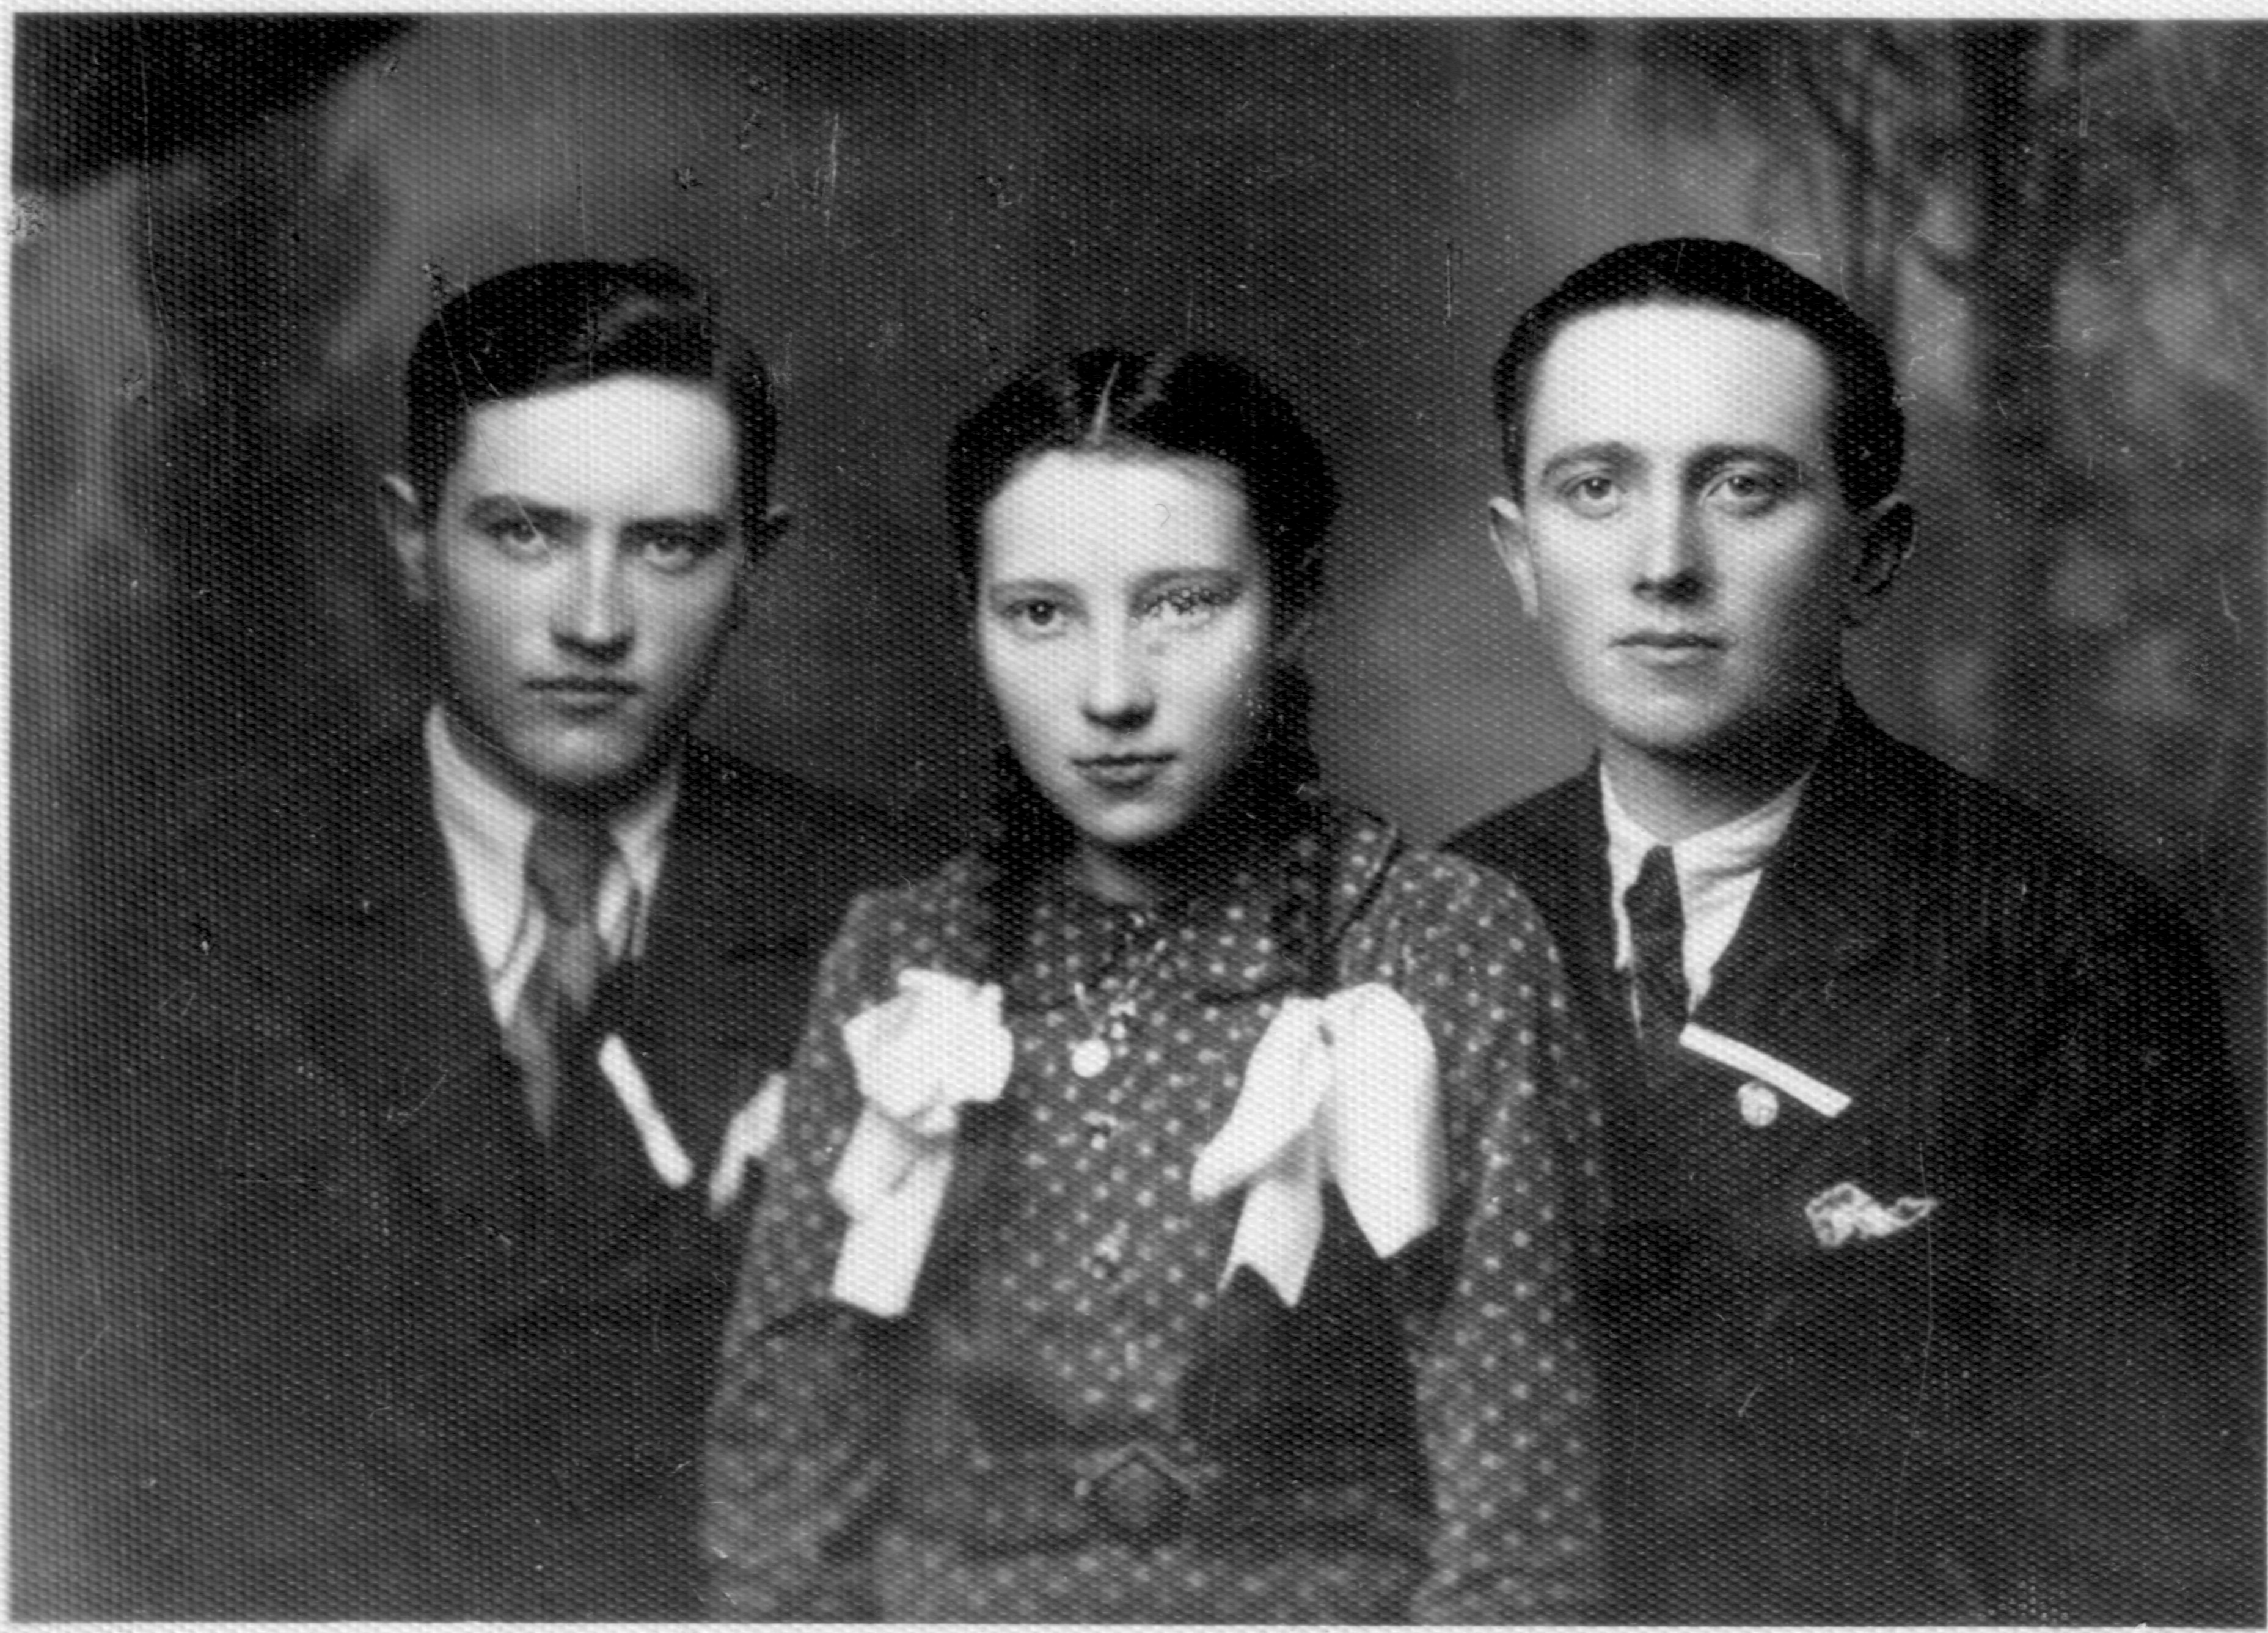
\includegraphics{../bilder/HeinzHansKaethe-b.jpg}
			
			\end{centering}
			\end{titlepage}

		
		

		{
				\setcounter{tocdepth}{3}
		\tableofcontents
					}
	
\begin{multicols}{3}
\textbf{Anmerkung des Protokollanten:} In Ungarn haben viele Orte wie so
oft in Osteuropa oder auch an der deutsch-französischen Sprachgrenze
mehrere Namensformen. Ortsnamen sind so wiedergegeben, wie Käthe sie
benutzt (zu benutzen scheint), dass heißt, Deutsch, wenn sie die
deutsche Variante sagt, und Ungarisch, wenn sie die ungarische Variante
nutzt. Der ungarische Name ist im Fließtext ohne Akzente und Ähnliches
wiedergegeben; die Fußnote der ersten Erwähnung gibt die richtige,
amtliche, ungarische Schreibweise wieder sowie die gebräuchliche(n)
deutsche(n) Schreibweise(n). Man beachte \emph{Bonyhad}: Sie nutzt fast
immer die ungarische Form, jedoch scheint sie an ein oder zwei Stellen
in das deutsche \emph{Bonnhardt} zu verfallen. Des Weiteren wurde
versucht, das Protokoll soweit wie möglich umgangssprachlich wortgetreu
zu halten, was weder durchgehend gelang noch immer möglich war.
Insbesondere die Verneinung „nicht“ wurde immer als „nicht“
wiedergegeben und Worte, die in der Umgangssprache typerweise
verschliffen werden, wie zum Beispiel „es“, wurden allermeistens voll
wiedergegeben. Teilweise habe ich auch aus anderen Gründen Stellen mehr
paraphrasiert denn protokolliert. Texte in eckigen Klammern sind
Präzisierungen oder auch Paraphrasen von Gesagtem.

Es sitzen im Raum, vermutlich um einen Tisch mit Fotos Käthe Klausch,
Schwester von Hans Hufnagel und Heinrich „Heini“ Hufnagel, ihr Mann
Friedrich, ihre Nichte, und Tochter von Hans Hufnagel, Ruth Gleichmann,
sowie deren Tochter Susanne.

\hypertarget{anekdoten}{%
\section{\texorpdfstring{Teil 1 \emph{Anekdoten} (54:55
Minuten)}{Teil 1 Anekdoten (54:55 Minuten)}}\label{anekdoten}}

\hypertarget{section}{%
\subsection{0:00}\label{section}}

\begin{description}
\tightlist
\item[Ruth]
Ich wusste nicht, wann die alle geboren sind.
\item[Käthe]
Das kann man ja noch machen. Also ihre Eltern, und der älteste Bruder,
das ist ja von der „Grill“-Käthe, in Mornshausen, nicht in Mornshausen,
wie heißt denn das
\item[Ruth]
Kombach
\item[Käthe]
– in Kombach gestorben ist, also Hoffmann, ist ihr Vater. Paar Tage,
nachdem der jüngste geboren war, ist er nach Kanada, und das war der Oma
ihr großes Vorbild – sie wollte nie heiraten, sie wollte auch nach
Kanada
\item[Ruth]
Also er von fünf Kinder abgehauen
\item[Käthe]
Ja nein, er ist nach Kanada, und hat gespart, und wollte seine Familie
nachholen, und sie war die einzigste {[}sic{]} Tochter und die Eltern
haben sie nicht gehen lassen. Und wie sie das Geld zusammen hatte,
musste sie in Etjasaschar bleiben.
\item[Ruth]
Also die Oma hat immer erzählt, das war so das, was sie im Kopf hatte:
„Er ist abgehauen von fünf Kindern und hat eine Frau mit fünf Kindern
sitzen gelassen“.
\item[Käthe]
Also so hat man's mir erzählt – das weiß ich nicht
\item[Ruth]
Das ist die Uroma, Susanne{[}?{]}
\item[Käthe]
Das ist meine Mutter, die Oma/Uroma
\item[Ruth]
Und die ist '97 {[}1897{]} geboren?
\item[Käthe]
Ja, und sie wollte nach Kanada, zu ihrem Bruder, und wollte nicht
heiraten. Und er hat – jeder Freier der kam – junger Bursche – hat sie
nein gesagt. Und da hat er eines Tages gesagt: „So, und wer jetzt kommt,
den musst du heiraten“. Und dann ist mein Vater gekommen. Wo sie sich
begegnet sind, ich weiß es net, und dann hat er gesagt „und den musst du
heiraten“. Und der stammte aus Hidasch\footnote{Hidas, deutsch
  \emph{Hidasch}, 2000-Einwohner-Nachbardorf von Bonyhad,
  \url{https://de.wikipedia.org/wiki/Hidas}}. Nachbargemeinde, früher
war das ja nicht so wie heute, das man genau wusste – das war ein
reicher Bauernsohn, das war sehr wichtig. Der hatte ja hier drei Söhne,
und mein Vater war der jüngste. Der älteste Sohn {[}unverständlich{]}
ist Großvater, ich nehme an, dass das seine Frau ist {[}vermutlich auf
ein Foto zeigend{]}. Ich hab sie nie kennengelernt. Und das ist der
älteste Sohn mit seiner Frau, auch ein Hufnagel, der mit den
{[}\ldots{}{]}-städtern mit seiner Frau. Das nächste ist der, der
Bräutigam mit der Braut –
\item[Ruth]
Ist das der Opa?
\item[Käthe]
Ja. Das ist der Heinrich, das ist der Hans, und das hier – ist der Opa
\item[Ruth]
Ach was
\item[Käthe]
Ja, der elegante ist der Opa
\item[Ruth]
Der sieht ja wiederum Susannes Opa, also meinem Vater ähnlich, hätte ich
nicht gedacht
\item[Susanne]
Das ist dein Opa – mit den Opabezeichnungen komme ich durcheinander
\item[Ruth]
Das ist mein Opa Melchior. Das Bild hab' ich noch nie gesehen
\item[Käthe]
Und zwar habe ich das von ihrer Schwiegertochter. Die hatten wir in
Hevis\footnote{Hévíz, deutsch \emph{Hevis}, Kurort am Balaton-Plattensee
  mit Thermalsee \url{https://de.wikipedia.org/wiki/H\%C3\%A9v\%C3\%ADz}}
getroffen, da waren wir zur Kur gewesen, und vorher hatten wir
telefoniert, und da hat sie gesagt: „Ich bring euch was mit“ und da
haben die {[}unverständlich{]} die alten Bilder mitgebracht und wir
haben die Bilder kopiert. Und so bin ich an dieses Bild gekommen. Und so
habe ich meinen Opa praktisch das erste Mal gesehen. Die Daten habe ich
hier aufgeschrieben. Da ist er nochmal. Und das ist sie.
\item[Ruth]
Deine Großeltern
\item[Käthe]
Meine Großeltern. \ldots{} Und zwar beide sind Bauern geworden. Und er
war Bürgermeister in Hidasch geworden, und ein ganz großes Gut, aber es
hat ihm nicht gereicht. Und er hat – so wie ein Rittergut – „Busta“ hat
man bei uns dazu gesagt – hat er gekauft. In {[}...{]} heißt das Busta,
und das ist in der Nähe von Fünfkirchen, Pecs\footnote{Pécs, sprich
  „Petsch“, deutsch \emph{Fünfkirchen},
  \url{https://de.wikipedia.org/wiki/P\%C3\%A9cs}: Regionalzentrum mit
  150~000 Einwohner, wechselhafter Geschichte der Türkenkriege}, in der
Nähe. Und dieser ehemalige Besitzer, der war total verschuldet, und da
war kein Grundbucheintrageinsicht, und er hat die ganzen Schulden
mitgekauft, und dadurch ist er bankrott gegangen, dann war garnix da.
Und weil mein Vater ja immer von Geburt {[}\ldots{}{]} hat man ihn nach
{[}\ldots{}{]} (das ist in der Nähe von {[}\ldots{}{]}) die Kreisstadt
geschickt. Da ist er in die {[}\ldots{}{]}, die Bürgerschule gegangen,
und hat ungarisch gelernt. Mein Vater, das war kein Dummer gewesen –
weil er die schwere Arbeit nicht leisten konnte. Und seine Mutter, die
war ja lungenkrank gewesen, und die ist hier – hab ich ja auch
aufgeschrieben – „Großvater Heinrich, geboren 1862, gestorben am
17.12.19{[}\ldots{}{]} in {[}\ldots{}{]}, ist 62 Jahre alt geworden.
Seine Frau, habe ich nicht gekannt, Hufnagel Grete, geborene Elfenbein,
habe ich auch nur 1868 in Gischmaniuk geboren, und gestorben am
29.4.1919 in Hidasch.
\item[Ruth]
Sieht aber so ein bisschen slawisch aus
\item[Käthe]
Sind ja Deutsche
\item[Ruth]
Slawisches Gesicht. Und die Oma war ein hübsches Mädchen
\item[Susanne]
Also da ist meine Uroma
\item[Ruth]
Ja
\item[Käthe]
Also das sind jetzt die Hoffmänner, Melchior seine Mutter und sein
Vater.
\item[Ruth]
Der Opa ist geboren {[}wann{]}?
\item[Käthe]
Der ist geboren 1892, am 16. Juli. Der hätte jetzt am 16. Juli
Geburtstag.
\item[Ruth]
Weißt du noch das Sterbedatum vom Opa?
\item[Käthe]
Ich hab es aufgeschrieben. Ich hab es sogar draußen in meinem Kalender
\end{description}

\ldots{}

\begin{description}
\tightlist
\item[Susanne]
Also es waren alles Deutsche, die in Ungarn gelebt haben? Die Hufnägel?
\item[Käthe]
Alles, alles. Und die Hoffmänner auch. Und zwar bin ich bei den
Hoffmännern sehr, sehr weit zurückgekommen und einen Hoffmann selbst
habe nicht \ldots{} {[}unklar{]} aber ein Nebenzweig, die Frau, die
einen Hoffmann geheiratet hat, die ist hier aus Idstadt gekommen.
\item[Friedrich]
19. 2. 1960 ist er gestorben
\item[Ruth]
Ist er noch 68 geworden, der Opa
\item[Käthe]
Die ist aus Idstadt, Da waren wir dort gewesen, und haben den Auszug
{[}vermutlich Kirchenbuchauszug{]} gesehen. Und wie sie ausgewandert ist
– 1720, im Siebzehnten {[}Achtzehnten{]} Jahrhundert damals. Und bei den
Hufnägeln bin ich leider Gottes nicht so weit zurückgekommen wie bei den
Hoffmännern, weil ich hätte gern gewusst: „Wo sind die Urwurzeln, von wo
sind sie hier ab“. Aber sind beide immer deutsch geblieben, da war nie
was Fremdes dazwischen. Also wenn du meinst –
\item[Ruth]
– Auch kein ungarisches Blut
\item[Käthe]
Gar nicht
\end{description}

{[}unverständlich{]}

\begin{description}
\tightlist
\item[Käthe]
Und das war deine Stieftante, das war ihre Hochzeit, und das ist ihr
Mann, der Wirt. Das ist die Eva, von der Eva Schüssler die Mutter,
\item[Käthe]
Und dann kam die Lissi-Tante, die in {[}\ldots{}{]} {[}Mehrholz{]}
gewohnt hat, das war die Lissi, und das ist der Heini {[}Bruder von Hans
Hufnagel{]}, der in Wien zum Schluss war. Sie war die jüngste. Und sie
ist ja auch schon früh verstorben.
\item[Ruth]
Meine Uroma ist auch schon früh gestorben.
\end{description}

\hypertarget{minuten}{%
\subsection{≈ 9 Minuten}\label{minuten}}

\begin{description}
\tightlist
\item[Käthe]
Ja, die habe ich auch nie gekannt, ich habe nie eine Oma gehabt. Eine
geborene Taubert war sie, Oma, geboren am 3.9.1867 in Bonyhad\footnote{Bonyhád,
  deutsch \emph{Bonnhard},
  \url{https://de.wikipedia.org/wiki/Bonyh\%C3\%A1d}: Lokales Zentrum
  der Herkunftsgegend der Familie Hufnagel, heute noch Schulort und
  Standort der weiterhin existierenden deutschen Selbstverwaltung},
gestorben am 27.6.1923 in Bonyhad. Und ich bin ja '28 geboren, habe sie
{[}daher{]} nie gesehen, nie eine Oma gehabt. Eine Oma streichelt
{[}ja{]}, und der Opa war ein ganz ganz strenger. Hat sämtliche
Enkelkinder mit seinem Krückstock verschlagen. Alle, nicht nur mich und
deinen Vater und den Heini, auch die anderen Kinder auch alle. Jeder hat
sich gefürchtet vor dem. Und zwar hat er – ich kenne ihn nur mit dem
Krückstock hier – er ist nach Wien gefahren mit den Pferden, was sie in
Wien wollten, weiß ich nicht. Als er da unterwegs von Bonyhad mit dem
Pferdefuhrwerk war nach Wien, und unterwegs sind die Pferde
durchgegangen, gescheut durch irgendwas und haben ihn mitgeschleift. Und
dadurch hat er ein steifes Bein behalten. {[}\ldots{}{]} Und diesen
Krückstock haben wir alle gefürchtet. Und wir sind nur zum Opa gegangen
– waren alle sehr religiös, vor jedem Essen musste gebetet werden, und
nach jedem Essen danke, aber gekloppt hat er uns alle, ob wir etwas
verbrochen hatten oder nicht verbrochen hatten, das war egal. Auf jeden
Falls sind wir nur hingegangen, wenn er Geburtstag hatte, dann mussten
wir immer ihm gratulieren und ein Gedicht aufsagen, das musste man. Da
sind wir nur pflichtbewusst hingegangen und haben gratuliert und dann
haben wir ein Geldstück von ihm gekriegt, das war unser ganzes Geschenk
im ganzen Leben, was wir vom Opa gekriegt hatten, wenn er Geburtstag
hatte, dann hat er uns immer ein Geldstück gegeben. Und noch eine
Geschichte dazu: Von den Hoffmännern, ob mütterlicherseits oder
väterlicherseits, das weiß ich jetzt nicht mehr, hat die Oma immer
erzählt – Taubert, muss von mütterlicherseits her sein – diese Oma war
so geizig gewesen, ihre Oma, die war so sehr geizig gewesen, sie ist
gestorben, und dann hat ihr Mann gesagt: „Jetzt darf ich mal mein
Frühstücksei alleine essen“. Die war so geizig, das Frühstücksei wurde
geteilt, Halbe Halbe, {[}\ldots{}{]} und wenn sie, Kinder, hingekommen
sind, und früher haben sie doch ihre Trachtröcke gehabt, und da war so
eine Tasche drin, und dann hat sie gesagt, ich kann mit meinen
Ellenbogen nicht in meine Tasche reingreifen, also es {[}sie?{]} hat für
die Kinder nichts abgegeben. Und wie sie gestorben war und der Opa hat
das gesagt „er darf jetzt endlich mal sein Frühstücksei alleine essen“,
da haben sie die Goldstücke gezählt. Geld auf dem Tisch gezählt, als
Erbe, und Silberstücke waren so viele, die haben sie dann mit der Waage
gewogen, um {[}sie{]} zu verteilen. Reich war sie, aber sattessen durfte
sich der Opa davon nicht. Ich habe sie nicht gekannt, ich kenne es nur
vom Erzählen. Das ist von der Oma. Und die Oma selbst, sie hat so schöne
Kleider gehabt, und die Lissitante wollte immer nur was sie {[}ihr?{]}
nicht gepasst hat, wollte sie haben. Ihre Eltern haben gesagt: „du bist
ja dumm! Die Kleider was deine Schwester hat, die willst du haben“ –
„Die will ich haben, ich will nix neues, die haben mir so gut gefallen“.
Und nachher, wie sie Melchior geheiratet hatte, und es hat sich
rausgestellt, dass er krank ist, dass er immer krank war, das wusste man
ja vorher nicht, und die Hufnägel haben das ja auch nicht gesagt, die
waren froh, dass sie beim jemand unter war, und dann fing natürlich für
sie die Notzeit an, zu mir hat sie mal gesagt: „Weißte, ich hätt' mich
so sehr im Leben gefreut, wenn dein Vater einmal heimgekommen wäre, und
hätt' mir mal Geld auf den Tisch gelegt, die Frau musste für die Kinder
sorgen, die musste für Essen sorgen, die musste für Geld sorgen, die
musste alles machen. Also, der Opa war krank, und mein Großvater hat ein
sehr großes Haus gehabt, ich habe mal gezählt, da waren zehn Einwohner
drin
\item[Ruth]
Der Hufnagel-Großvater?
\item[Käthe]
Der Hoffmann-Großvater. Da waren natürlich nicht solche Riesenräume, da
gab es ein Zimmer und eine Küche, das war alles. Und Bad gab es ja
früher nicht, um 1800 in den Räumen, da waren im Hof {[}waren{]}
Toilettenbatterien, und die mussten dann immer wieder, wenn es voll war,
mussten die geleert {[}werden{]} Da war für die Herrschaften, der Opa
und für seine Familie, die haben ein Extraklo gehabt, und für alle
anderen Leute die dadrin gewohnt haben gab es das Sammelklo, und jeder
musste halt warten, wenn {[}wann, bis wann{]} er da drauf konnte. Und
was wollt' ich jetzt erzählen? Ja, mit der Oma. Die Oma, die musste
natürlich – das bisschen Landwirtschaft was sie hatten, was natürlich
nicht gereicht hat, und die hat dann einen Teil vom Opa, von ihrem Mann,
da war eine Tante gewesen, und die hat denen was zukommen lassen, so hat
die Oma auch etwas gekriegt, und konnte in {[}den{]} Altgeberg\footnote{Altgeberg:
  Fast schon anekdotischer Name des Wohnorts meiner Urgroßeltern in
  Ungarn, gemeint ist ein etwas abseits gelegenes Wohngebiet \emph{bei},
  aber nicht in, Bonyhad} – das war außerhalb von Bonyhad – ist ein
Weinberg, ein großer Weinberg, da sind so Presshäuser und so kleine
Wohnungen dabei, mit dem Weinberg dabei, ein großer Obstgarten, und
hinten anschließend war noch ein großes Feld, wo man noch alles Mögliche
anbauen konnte. Da hat sie so eins erworben, und das war dann ihr
Lebensunterhalt, da hat sie Obst, Gemüse, Obst hatten wir alles gehabt,
von der Frühkirsche angefangen, bis alles, was es an Obst gab, hatten
wir gehabt. Dann hat die Oma das genommen und auf den Wochenmarkt
getragen, mit so einem großen Korb auf dem Kopf, da hat sie ein paar
Pfennig bekommen, und das hat halt auch nicht gereicht. Und dann gab's
einen Jude', Kohn hieß der, das war ein Eierhändler, und für den ist sie
auf die Ortschaften raus, die Bauern haben ja alle viel' Hühner gehabt,
es waren ja alles Naturhühner, nicht so Batterien wie heute, und aber
das musste ja beigetragen werden, und da hat sie die Eier aufgekauft,
und hat am Anfang so einen Korb voll Eier heimgetragen von zig
Ortschaften ringsum
\item[Ruth]
Auf dem Kopf
\item[Käthe]
Auf dem Kopf heimgetragen, und dann konnte sie das nimmer, und dann
wurde bei einem Bauer ausgehandelt, wo sie die hinstellen durfte, die
Eier, die Sammelstelle, da hat sie die zusammengetragen und alle dahin
gebracht und dann wurden sie abgeholt, aber sie musste den Weg – alles,
Ortschaften, es war ja nicht so, das eine Ortschaft bei der anderen war,
da waren ja zwölf oder noch mehr Kilometer dazwischen. Alles dahin
laufen, abklappern, und das hat sie alles noch nebenbei gemacht und hat
uns Kinder noch versorgt, muss man sich mal vorstellen
\item[Ruth]
Hat sich das denn gelohnt, mit den Eiern?
\item[Käthe]
Ja sicher. Die konnte\ldots{} es waren ihre Einnahmen, ja das andere hat
ja nicht gereicht.
\item[Ruth]
Was hat der Opa {[}Opa Melchior, es geht immer noch um Käthes Vater{]}
gemacht, sach mal?
\item[Käthe]
Der war krank.
\item[Ruth]
Wie war er krank?
\end{description}

{[}Nicht gut verständliches Geplänkel, in etwa „hat er nur da gesessen,
hat er nichts gemacht?“{]}

\begin{description}
\tightlist
\item[Käthe]
Ja, ich hab meiner Mutter auch mal gesagt: „Wenn der Papa koche' tut –“,
der „Vater“, wir haben ja Vater gesagt, „– der kocht dann viel besser
wie du“. Hat sie gesagt: „Ja, der greift ja auch in die Volle{[}n{]}
rein, ich muss es einteile' und sparen“. Nicht, also er hat auch schon
mal gekocht, aber das er sonst – und was er immer gemacht hat, er hat
immer die Schuhe geputzt von uns allen. Die Schuhe hat er auf Hochglanz
gebracht, aber das er sonst etwas gemacht hätte – doch, er konnte sehr
gut Obst veredeln, wenn so ein neuer Spross ist, ein Wildspross, der
muss ja veredelt werden, das konnte er sehr gut. Und wenn im Weinberg
die Zeit war, wenn die Reben da treiben, dann müssen die gebunden
werden, da gab es früher Raffia{[}?{]}, heute ist es einfacher, da gibt
es so eine Schusspistole, die macht klack, klack, klack, und dann ist so
ein Trieb gefestigt, und da waren ja damals nicht so Treter wie heute,
sondern da war ein Stock dabei, so ein Stab, und der musste da
festgebunden werden. Und da hat er geholfen. Aber sonst habe ich meinen
Vater nie was sehe', dass er was gemacht hat. Er konnte auch nicht, denn
er war wirklich sehr krank. Der hat eine Seite gar keine Lunge mehr
gehabt, auf der anderen Seite nur noch ein Restchen. Und das sie damit –
\item[Ruth]
Hatte der zu wenig Sauerstoff?
\item[Käthe]
– Atemnot hatte, und hat gar keine Luft bekommen, das ist eine
seltene\ldots{} Aber das weiß man als Kind auch nicht, und trotzdem:
Keines von uns Kindern ist krank geworden.
\item[Ruth]
Hatte der nur eine TB {[}Tuberkulose?{]}
\item[Käthe]
Hatte TB, {[}\ldots{}{]} seine Mutter ist an Tuberkulose gestorben, mit
jungen Jahren, haben wir ja das Datum hier, wann sie gestorben ist.
Hufnagel, Gretel, hier: 1868 geboren, 1919 ist sie aber 51 Jahre alt,
ist sie schon gestorben. Sie hat – mein Vater hat – seine Mutter hat
Tuberkulose gehabt. Und sein Vater wollt' wenig von ihm wissen, weil er
war ja kein kräftiger, starker Mann, er war ein Kümmerling gewesen,
nicht, und den kann man ja in einer starken Familie schlecht gebrauchen,
ja, und sie hat halt die Hand über ihren jüngsten Sohn gehalten, das war
halt ein großer Halt gewesen.
\item[Ruth]
Aber die Oma\ldots{} waren die dann von der Familie aus sehr reich? Oder
hatten die gut Geld? Weil du sagt, die war immer so gut angezogen und
so?
\item[Käthe]
Er war Maurer
\item[Ruth]
Der Opa war Maurer
\end{description}

\hypertarget{minuten-1}{%
\subsection{≈ 19 Minuten}\label{minuten-1}}

\begin{description}
\tightlist
\item[Käthe]
Der war Maurer. Und zu der Maurergeschichte muss ich auch noch was
sagen. Und zwar hat er nicht nur für sich, in so einem großen Haus gab
es ja immer genug zu tun, also fleißig war er, sondern hat auch bei
anderen Aufträge gehabt, nicht immer große Häuser, sondern was
auszubessern, oder Kleinigkeiten zu mauern, und da ist er, hat er mal
bei einem Schuster gemauert. Und der war so arm gewesen, der
Schuhmacher. Und früher war das so, dass wenn ein Handwerker kam, da
wurde der durch den, für den er gearbeitet hat, der musste den an dem
Tag verköstigen. Und dann war er dort gewesen, und der Schuster hat
einen Lehrjungen gehabt, und dann hat er gesagt: „Gell Meister, jetzt
arbeiten wir tüchtig, und wenn wir Geld haben, dann gehen wir auf den
MArkt, in Bonyhad gab es einen Jahrmarkt, der war zweimal im Jahr, der
war außerhalb von Bonyhad, mit Karussell, und mit Schaustellern, und
weil natürlich die ganzen\ldots{} sonst gab es nichts – dann kann man
sich natürlich vorstellen, dass das ein Mordsanziehungspunkt war, und
der ganze Kreis kam zusammen. Und da hat der Bub gesagt: „Dann gehen wir
dahin, und dann kaufen wir uns ein Futzje\footnote{Nachgucken}, und das
kleine Futzje, das füttern wir, bis es groß und fett ist, und dann
schlachten wir es, aber gell Meister, dann essen wir Wurst ohne Brot.“
Und hat der Meister gesagt, der {[}den{]} Gürtel genommen von seiner
Hose: „Was Wankerl\footnote{} {[}vermutlich dialektal, verwandt mit
engl. „wanker“{]}, du willst Wurst essen ohne Brot“ und hat ihn mit dem
Riemen {[}dem Gürtel{]} versohlt. Und es war kein Geld, das Futzje zu
kaufen, aber hat schon die Schläge gekriegt. Da hat der Opa gesagt zu
seiner Frau: „Ich ess' da nix mehr, die haben ja selbst nichts zu essen,
ich komm' heim zum essen“ Der Papa hat die Geschichte erzählt, hat
nichts weiter zu erzählt. Also so reich sind die gewesen. Ja, es war
eine arme Zeit. Die Oma hat mir auch erzählt, dass ihre Großmutter,
eine, ob es jetzt die geizige war oder die andere weiß ich nicht, die
sind rausgefahren, des muss\ldots{} die sind ja 1720 hingekommen, also
so 1790 oder vielleicht 1800 Anfang war es rum – rausgefahren und haben
im Winter hat es {[}das{]} Brennholz nicht gereicht, und da mussten sie
Brennholz draußen holen, und dann hat der Großvater, also ihr Großvater
schon ein Fohlen gehabt, hat er hinne angebunden, und ist rausgefahren,
weil es die Wölfe gab, war ja alles voller Wölfe, und da sind sie
rausgefahren und haben das Holz aufgeladen, es ging alles gut, aber dann
auf der Heimfahrt kam ein Wolfsrudel angebraust, und da hat er auf die
Pferde heim hat es nicht gepackt und dann haben sie das Fohlen, das sie
vorher extra mitgenommen, das haben sie geopfert, sonst wären sie
überfallen worden von dem Rudel, so sind sie heimgekommen. Und die Oma
selber hat erzählt, dass ihr{[}e{]} Großmutter – eines Tages hat sie die
Fenster offen gehabt, und ht rausgeguckt, und da steht draußen der Wolf,
die Pfoten aufs {[}\ldots{}{]} und guckt rein. Die Wölfe tun heute ja
nix mehr, die haben ja damals nur die Menschen gefressen, aber heute
nicht
\item[Ruth (lachend)]
Heute nicht mehr, gell?
\item[Käthe]
Ja nein, die dürfen ja heute wieder kommen als Ansiedler. Ich sage, es
geht mir gut, ich tu dir nix. Und dann ist bei uns der Kalvarienberg
{[}sie spricht „Kalfarien“{]}\footnote{„Kalvarienberg, auch
  Stationsberg, ist die Bezeichnung für umfangreiche Nachbildungen der
  Passion Christi, die als Andachts- und Wallfahrtstätten dienen.“
  \url{https://de.wikipedia.org/wiki/Kalvarienberg}}, das ist die
Straße, wenn man nach Sechsard\footnote{\emph{Szekszárd}, deutsch
  \emph{Sechshard} oder \emph{Sechsard},
  \url{https://de.wikipedia.org/wiki/Szeksz\%C3\%A1rd}} fährt –
Sechshard, das hat' ich vorher schon, unsere Kreisstadt, da ist der ist
ein Kalvarienberg, das ist ein Kreuz, ein hoher Sockel, und da ist ein
Kreuz oben drauf, und da ist der Schornsteinfeger von Bonyhad, ist
gegangen, im Winter, war auch die Winterzeit, um im Nachbarort
Schornsteine zu fegen, oder irgendwas, auf jeden Fall kamen die Wölfe an
und er wusste nicht mehr, wie's {[}wie man{]} auf den Sockel da drauf,
und hat sich da auch mit seinem Zeug da festgeschnallt, denn es war ja
Winter und klirrende Kälte, war ja mehr kalt wie noch heute, und am
nächsten Tage sind die Leute da vorbeigekommen, und die Wölfe haben
unten gehockt und sind nicht weggegangen und der Mann ist oben erfroren.
Am nächsten Tag sind die Leute gekommen\ldots{} Wir mussten in der
Schule mal jeder von seiner Gemeinde was schreiben, und da habe ich
diese Geschichte auch reingeschrieben, und zwar habe ich die auch so
Sachen\ldots{} bei uns gab es die Spinnstuben in der Winterzeit
\item[Ruth]
Die gab es noch bei euch?
\item[Käthe]
Die gab's, und das ist schön. Da gab es ein Spinnrad – die Oma hatte ja
eines mitgebracht, das hat glaube ich dein Bruder Hans genommen
\item[Ruth]
Ich weiß es nicht
\item[Käthe]
Der hatte Interesse gehabt dadran, der Hans – ist ja egal, wo es
geblieben ist, jedenfalls da hat sie Wolle gesponne, oder Hanf
gesponnen, und dann ist man mit den Nachbarn zusammen gekommen, da
wusste man: wir treffen uns jetzt mit dem Nachbarn, die kommen zu uns,
und dann wurde vorher gebacken, für den Abend, und dann hat man da
zusammengesessen, da wurden Geschichten erzählt, und wir Kinder, wir
Mädchen, oder Nachbarmädchen, die ja auch in Russland {[}Ungarn{]}
geblieben ist, die Weber-Lissy\footnote{nachfragen}. Wir haben gespielt,
oder \ldots{} wurde viel gestickt bei uns, viel Handarbeit gemacht. Und
dann wurden immer so Geschichten erzählt. Da hat man natürlich immer
gehorcht, nicht. Und da sind auch so Geschichten mit den Wölfen und so
Sachen zum Vorschein gekommen, es war sehr schön. Und da gab's heißen
Tee zu trinken, und die Erwachsenen haben einen Punsch getrunken, einen
Glühwein, nicht, aber wir haben einen Teet gekriegt und waren seelig und
vergnügt, da hat keiner ans Schlafegehe gedacht, es waren schöne Sachen,
und die gab's in der Winterzeit, ja.
\item[Ruth]
Und wann hat die Oma jetzt geheiratet? {[}ihre Oma, Katharina
Hufnagel?{]} Wann haben die sich kennengelernt? Die Oma war ja noch
jung?
\item[Käthe]
Die Oma war 23.
\item[Ruth]
Ach doch schon 23.
\item[Käthe]
Weil sie ist ja 1897 geboren, und 1920 hat sie geheiratet. 20. Mai 1920
hat sie geheiratet. Die Oma war arm dran, ein Leben lang, und sehr
bescheiden. Und dadurch, dass sie so zurückstecken musste – man muss
sich vorstellen, vorher ging es ihr gut, und dann, in der Ehe, ging
alles rückwärts, und überall war Not und Elend, und drei Kinder waren
da, und da war das nicht einfach für sie, und dein Mann hat mal gesagt –
\item[Ruth]
Mit 23 hat sie geheiratet, im Mai.
\item[Käthe]
Sie war 23 Jahre alt.
\item[Ruth]
Ja, dann sind ihre Kinder bald gekommen
\item[Käthe]
Ja, natürlich, der Heini sofort, obwohl sie ein altes Mädchen war. Die
haben ja früher, guck mal, die haben ja früher – ihre Schwester, die war
in dem Alter schon längst Witwe von drei Kindern. Die haben alle\ldots{}
die sind aus der Schule gekommen und sind sofort
\item[Ruth]
Die Wirthstante? Die war so früh Witwe?
\item[Käthe]
Ja ja, das ist ihr Mann, der war im 14/18-Krieg {[}Sie meint den Ersten
Weltkrieg{]} und ist 1919 schon verstorben, und da hat sie schon drei
Kinder gehabt. Die Kathi, die auch schon so schnell verstorben ist – wie
die Russe' kamen, gab's kein Arzt, keine Medikamente, war krank, eine
Grippe gehabt, ist umgefallen und war tot – das war auch ein\,Schock.
Und ihr Sohn, der Hans, der ist im zweiten Krieg {[}Zweiten
Weltkrieg{]}, der war bei der {[}unverständlich{]}, bei der {[}dem{]}
ungarischen Militär – dein Vater und der Heini, die hätten ja auch zum
Militär gemüsst, da sind sie lieber zu den Deutschen gegangen als zu den
Ungarn, zur UNRI\footnote{nachfragen}, und der ist nach Russland
gekommen und man hat nie was dem gehört, bis heute nicht. Vermisst. Ob
er umgekommen ist oder in Gefangenschaft gekommen ist, man weiß das
alles nicht
\item[Ruth]
Kannst du nochmal was vom Papa erzählen, wie der aufgewachsen ist? Was
er alles so an Ausbildung gemacht hat? Oder als er bei seinem Großvater
war?
\item[Käthe]
Ich kann gar nicht mal allzu viel erzählen. Guck mal, wir sind fast
sieben Jahre Unterschied, und damals war das ja so, der ist bis zum
zwölften Lebensjahr~– ist man zur Schule gegangen, bis zur Sechsten, und
dann war Schluss, und dann gab es die Wiederholungsschule, gab's dann,
wo man zweimal zur Woche nur zur Schule gegangen ist, eine
Wiederholungsschule hieß das damals.
\item[Ruth]
Das war eine deutsche Schule? Oder ungarisch?
\item[Käthe]
Ungarisch. Und sein Lehrer, der hat damals gesagt, meine Kinder, die
Deutschen, die aus meiner Klasse rauskommen, die werden keine deutsche
Zeitung lesen können. Das war dem sein Vorsatz –
\item[Ruth]
Der wollte, dass die nur Ungarisch können.
\item[Käthe]
Genau, und dann kannst du dir vorstellen, wenn da die Schrift und das
Lesen nicht so war, das war nur das bisschen, was er von daheim von
den\,Eltern mitbekommen haben, das andere von der Schule war bewusst die
sollten keine deutsche Zeitung lesen, so war das gewesen. Und dein
Vater, der war ein Luftikus gewesen. Hans in allen Gassen, der hat alle
Streiche gemacht, hat die Oma erzählt, der wollte nicht zur Schule
gehen, und dann ist er auf die Bäume geklettert, und hat von oben
Gesichter gemacht, und {[}\ldots{}{]} und sie stand unten mit einem
Besen und hat gedroht, und er hat sie ausgelacht, aber auf jeden Fall,
er ist zur Schule gegangen, und er war sehr geschickt, er hat – ich weiß
nicht, ich habe es leider Gottes nicht, habe ich schon ein paar Mal dran
gedacht, er hat in der Schule, das war so buntes Papier, so wie es heute
auch so Bastelpapier gibt, und da so verschiedene Muster haben die
dareingemacht, und da hat er so mehrere Packen gemacht, also er hat das
sehr gut gemacht, und das hatten wir daheim, das war was Kostbares,
aufgehoben, bis wir weg mussten {[}gemeint ist die Vertreibung{]},
solang haben wir das gehabt. Und dann, was er auch mir immer gemacht
hat, Ostern gab es immer ein Nestchen draußen, im Hof, wir hatten ja
viel Platz gehabt, und da sind wir Weidenruten gegangen, unten am Bach,
Weidenruten holen, Stäbchen, und da so Stöckchen reingemacht, ich konnte
es ja noch nicht so, aber er hat mir da immer geholfen, und hat so
Stöckchen rein, das geflochten, und dann sind wir losgegangen, und haben
Moos gesucht
\end{description}

\hypertarget{section-1}{%
\subsection{29:40}\label{section-1}}

\begin{description}
\tightlist
\item[Ruth]
Das hat der für uns auch noch gemacht. Als ich klein war kann ich mich
erinnern. Das kannte ich so sonst gar nicht mehr, und hat richtig was
festgeflochten
\item[Käthe]
Ja, immer Moos, lang vor Ostern musste das ja immer schon gemacht
werden, da war das schon wieder vertrocknet, dann ist er wieder
gegangen, wieder neues\ldots{} der Organisator war dein Vater. Und damit
da, wenn Regen ist, da nichts rein kommt, der hat der sogar einen
Verschluss obendrüber gemacht, so einen Deckel obendrauf, aber nicht so
glatt, sondern so eine Wölbung, dass, wenn der Osterhase da was
reinlegt\ldots{} {[}nichts kaputt geht{]} der wusste ja genauestens über
den Osterhasen bescheid \ldots{} Bis ich mal mittags schlafen gegangen,
bin rausgekommen, ein bisschen früher als sonst, dann waren sie am
Eierfärben gewesen, und da wusste ich, wer der Osterhase war. Aber dein
Vater, wie der noch so klein war, da hat der auch noch an den Osterhasen
geglaubt. Und da haben wir ja schon draußen am Altgeberg gewohnt, und
geht morgens raus, um nach dem Osterhasen, nach dem Nestchen, ob der
Osterhase schon da war, zu gucken, kommt da gerade ein Feldhase vorbei.
Und der Hansen: „Ei Häschen, bleibt doch stehen, ich bin doch da“. Das
war dein Vater gewesen. {[}Als er mit der Schule fertig war{]}
\item[Ruth]
Weißt du, wie alt er da war?
\item[Käthe]
{[}Er dürfte nicht älter als 13,14 gewesen sein{]}, da ist er zum Bauern
gekommen, und auf dem Bauern ging's ihm sehr, sehr schlecht, aber das
wusste man auch nicht. Und zwar haben die auch die Kinder genommen, von
minderbemittelten, wollen wir mal so sagen, und haben die Kinder richtig
ausgenutzt. Der musste schon früh aufstehen, und musste den Stall
ausmisten, und das Vieh versorgen, und hat wenig zu essen gekriegt, und
musste in so einer, dürftigen, alten Kammer schlafen, bis die Oma ihn
damals\ldots{} ihn da aufgesucht hat, und mitbekommen hat, dass es dem
Bub wirklich so schlecht ging {[}\ldots{}{]} und da hat sie ihn sofort
mit nach Hause genommen, und dann, hat die einen Bäcker gehabt – bei uns
in Bonyhad hat es drei Bäckereien gehabt, und – da ging es ihm auch
nicht gut, überkleg dir mal: Die jungen Burschen, die Lehrlinge, die
mussten abends um elf Uhr anfangen, Brot zu backen, der Ofen wurde
sauber gemacht, und angeheizt, und bis das alles fertig war in der
Zwischenzeit den Teig machen, und die Brötchen machen, Kipfel {[}?{]}
haben wir gesagt zu den Hörnchen, die waren ganz wunderbar. Und das
alles mussten die Abends um 11~Uhr, wenn die andere Jugend noch
Benedeni{[}?{]} und zusammen ist, da musste er schon in der Backstube
stehen, die ganze Nacht. Und morgens, wenn sie dann fertig waren, und
dann musste er noch – da gab es ja noch die Herrschaften, die die
Brötchen im Sack daheim hinbekomen haben – musste die Brötchen
ausfahren. Dann durfte er erst heimgehen, schlafen. Überleg' dir mal,
das war keine schöne Zeit.
\end{description}

{[}\ldots{}{]}

\begin{description}
\tightlist
\item[Käthe]
Und das als junger Mensch.
\item[Friedrich (ironisch)]
Die gute alte Zeit
\item[Käthe]
Die gute alte Zeit, ja.
\item[Ruth]
Gut sag mal, war eigentlich auch mal beim Opa, bei dem Hoffmannopa, eine
Zeit lang untergebracht?
\item[Käthe]
Ja, da waren wir alle mal gewesen. {[}\ldots{}{]} Mein Vater, und sein
Schwiegervater, die haben sich ja nattürlich nicht verstanden, weil der
{[}Balthasar Hufnagel{]} nichts gebracht hat, keine Leistung gebracht
hat. Da wollte er\ldots{} Seine Tochter hatte er vorher zu der Ehe
gezwungen, „du musst den heiraten“, und nachher, wie er krank war, wie
er mitbekommen hat, dass er krank ist, hat gesagt, „jetzt wird sich
geschieden“. Und da hat Mutter gesagt: „Ich habe vor Herrgott
geschworen, ‚in guten wie in schlechten Zeiten‘, ich hab' den Schwur
geleistet, ich bleibe dabei, ich muss das tragen, das ist mir auferlegt.
Nicht, und so hat sie das auf sich genommen, aber das war halt getrübt,
zwischen Schwiegersohn und Schwiegervater. Und da waren wir eine Zeit
lang. Die Lissitante war verheiratet, nach Meginitsch, geheiratet hat
die in Hollenbach, und da war der Opa alleine. Und natürlich, war
sowieso sein Liebling gewesen, und dann hat er sie reingeholt, und dann
waraen wir dort gewesen. Und der Hansen und der Heini, die mussten dann
auch bei ihm alle Arbeiten verrichten.
\item[Ruth]
Das hat der Papa auch manchmal erzählt, dass ihn der Opa auch geschlagen
hat(?)
\item[Käthe]
Ja
\item[Ruth]
Und dass er, morgens früh in den Stall musste, und dann in den
stinkenden Stallklamotten in die Schule, und in der Schule haben sie ihn
ausgelacht, weil er so gestunken hat. Und keiner hat ihm gesagt, er
müsste sich waschen oder so. Der ist aus dem Kuhstall in die Schule
gegangen. Oder Schweinestall, ich weiß nicht was die hatten.
\item[Käthe]
Der hat Kühe gehabt, und Schweine, ja.
\item[Ruth]
Und wie lange waren die da, bei dem Opa? Oder wie lange wart ihr da, als
Familie?
\item[Käthe]
Weiß ich nicht. Nicht allzu lange, wir waren eine Zeit dort. {[}Weil es
ja nicht lange gut ging mit den Kindern{]} – ich habe ja auch meine
Dresche von ihm gekriegt. Die Hoffmänner {[}auch{]}, der war nicht
einfach. Und dann war auch – wie er beim Bäcker weggekommen ist, weiß
ich nicht – eine Zeit lang in einer Keksfabrik gearbeitet.
\item[Ruth]
Das habe ich noch nicht gehört.
\item[Käthe]
In einer Keksfabrik. Und da hat er diese Bruchkekse mit nach hause
nehmen können. Sowas gutes habe ich mein Leben nicht mehr gegessen.
Weißt du, dass war ja was ganz besonderes, frisch gebacken, die Kekse.
So richtig so wie die Balsenkekse, so die Form war das gewesen. Da gab
es so eine Fabrik in Bonnhard, da war er gewesen, bis er dann zum
Militär gekommen ist.
\item[Ruth]
Hat er nicht auch noch etwas mit Maurer gemacht? Hat er nicht noch eine
Maurerlehre gemacht?
\item[Käthe]
Dasd war der Heini.
\end{description}

{[}Sinngemäß ob sie sich sicher sei{]}

\begin{description}
\tightlist
\item[Käthe]
Kann ich mich nicht erinnern. Ich weiß nur noch eines, die Oma hat auch
mal zwischenzeitlich mit Zucker gehandelt, so Bonbons. Und da hat sie
auch so mit Großware sich kommen lassen und die dann verkauft und da hat
sie dieses Sortiment in der guten Stubb' – gab ja eine gute Stub' – ein
Paradezimmer war das gewesen
\item[Ruth]
Wohnzimmer, wo keiner rein durfte. Das hatten wir auch noch.
\item[Käthe]
Da hatten wir drei Kleiderschränke gehabt. Drei große Kleiderschränke
und nur eine Kommode noch. Und auf den Kleiderschränken obendrauf hat
dann die Oma die Schachteln mit den Bonbons gehabt. Und dann ist die mal
heimgekommen {[}\ldots{}{]} – war ich wahrscheinlich ganz klein – auf
jeden Fall haben die Buben obengesessen, haben die Bonbons runtergeholt.
Der Hans – dumm war er nicht – hat einen Schirm genommen, aufgespannt
und damit heruntergezogen. Mit dem Stuhl ist er gar nicht rangekommen,
aber mit dem Schirm, und dann haben die unten gesessen, und haben
Bonbons gehabt. {[}\ldots{}{]} Also das war vielleicht nach der
Eiersache {[}\ldots{}{]}, also wie da die Zusammenhänge sind, so
chronologisch, kann ich nicht genau sagen, das sind ja nur Bruchstücke.
\item[Ruth]
War vielleicht auch frühkindliche Prägung. Der Papa hat noch als alter
Mann unheimlich gerne Bonbons gegessen, und wenn ich kam, dann kriegte
ich Bonbons in die Hand gedrückt, ob ich nun 50 war oder 55, aber ich
kriegte meine Bonbons.
\item[Käthe]
Siehst du mal, es war ja auch was besonderes.
\item[Friedrich]
Ist genauso. Da sind die Bonbons draußen.
\item[Käthe]
Und dann der Krieg, da ist er nur ein einziges Mal heimgekommen im
Urlaub.
\item[Ruth]
Er hat sich freiwillig gemeldet, bei den Deutschen.
\item[Käthe]
Er musste ja sowieso gehen.
\item[Ruth]
Er hätte zu den Deutschen gemusst?
\item[Käthe]
Zu den ungarischen\footnote{Käthe bezieht sich hier auf das
  Anwerbungsabkommen der SS mit der (ebenfalls faschistischen)
  ungarischen Pfeilkreuzlerregierung, dass Volksdeutsche aus Ungarn
  ihren (verpflichtenden) Wehrdienst auch in der Waffen-SS ableisten
  konnten. Hintergrund war, dass der SS bald nach der Machtübernahme die
  Rekrutierung im reichsdeutschen Inland verboten wurde, um die
  Rivalität mit der Wehrmacht zu dämpfen.

  \begin{itemize}
  \tightlist
  \item
    \url{https://de.wikipedia.org/wiki/Ausl\%C3\%A4ndische_Freiwillige_der_Waffen-SS\#Ungarn}
  \item
    \url{https://de.wikipedia.org/wiki/Ausl\%C3\%A4ndische_Freiwillige_der_Waffen-SS}
  \item
    \url{https://de.wikipedia.org/wiki/Volksdeutsche\#Volksdeutsche_in_der_Waffen-SS}
  \end{itemize}}. Und da sind sie beide – der Heini hat sich zuerst
gemeldet – und da hat er ihn mitgezogen. Der Hans wollte eigentlich noch
nicht gehen. Aber weil sein Bruder – die beiden waren ja unzertrennlich,
waren ja immer zusammen. Und der Heini, der hat ja als Kind nicht
gestottert, sondern er in einem gewissen Alter – ich ging noch nicht zur
Schule – da kamen in Sechsard, im Krankenhaus, da haben wir ihn besucht.
Und da hieß es, er hat Hirnhautentzündung, und da hat man auch gesehen,
er hat hinten eine Narbe gehabt. {[}\ldots{} Hirnhaut \ldots{}{]} Und da
danach hat er angefangen zu stottern, nach dieser Hirnhautentzündung,
vorher war er vollkommen normal –
\end{description}

\begin{description}
\tightlist
\item[Ruth]
– oder auch wegen dem Krankenhausaufenthalt, es kann auch sein, dass es
diese Trennung war
\item[Käthe]
In einem der Krankenhausaufenthalte war es so beliebt{[}?{]}, dass sie
zu Fuß – das sind 20, 30 Kilometer oder noch mehr – vom Bonyhad nach
Sechsard gelaufen und die mussten ja auch wieder zurücklaufen, an einem
Tag, sind wir nach Sechsard, der Opa, der Melchior, meine Mutter und
ich. Der Heini war im Krankenhaus und der Hans, der war damals
vielleicht – ich weiß es nicht, wo er war. Auf jeden Fall haben wir ihn
da besucht, und ich habe ihm – das Krankhaus, da war so ein schöner
Park, und an seinem Bett, {[}\ldots{}{]} So Hörgeräte mit Musik
\end{description}

\hypertarget{section-2}{%
\subsection{40:21}\label{section-2}}

\begin{description}
\tightlist
\item[Ruth]
Gab es das schon?
\item[Käthe]
Habe ich noch nie in meinem Leben gesehen gehabt, was für mich natürlich
was ganz besonderes gewesen ist, und ich wollte nur das im Kopf haben.
Und den Heini haben wir besucht, und er war in der Küche, und dann haben
die Frauen dort gesagt: „Den behalten wir hier, der ist so fleißig, der
geht und räumt bei den Patienten das Geschirr ab, und der ist ein
Fleißiger“. Und an dem Tag, wo wir ihn besucht haben, da war er auch aus
und hat geholfen. Wie wir dann heim gegangen sind, konnte ich nicht
mehr, und dann hat mich meine Mutter auf den Rücken genommen – wie ich
die Stella-Melanie {[}ihre Adoptivtochter{]} auch auf dem Rücken hatte –
weil ich nicht mehr konnte. 20 Kilometer heimlaufen, überleg' dir mal.
{[}Das kann man sich heutzutage nicht mehr vorstellen{]} Aber dadurch
ist man eingelaufen, überleg dir mal. Aber vom Hans damals, ich habe da
überhaupt keine Erinnerung. Weißte. Guck mal, ich bin auch von meiner
Mutter viel zu früh weggekommen, da war ich 16, wie der Russe kam. Da
bin ich schon weg.
\item[Ruth]
Dann bist du in die Schule?
\item[Käthe]
Dann bin ich geflüchtet.
\item[Ruth]
Aber wann bist du in die Schule? Bist du da jeden Tag hin- und
hergefahren, in die Schule?
\item[Käthe]
Ich bin gelaufen
\end{description}

{[}Ruth sich nach der Schulform erkundigend{]}

\begin{description}
\tightlist
\item[Käthe]
Da bin ich mit dem Fahrrad. Erst gelaufen, und das Fahrrad musste ich
mir erst verdienen. Gymnasium war ich nicht. Mittelschule {[}heute
Haupt- und Realschule{]}. Ich bin die ersten zwei Jahre gegangen, und
das dritte Jahr. Und im vierten Jahr hat meine Mutter gesagt, so, du
bleibst zuhaus', dann musst du nicht mehr gehen. Dann ist die Lehrerin
zu uns gekommen und hat gesagt: „das ist jetzt das letzte Jahr, und dann
hat sie ein Abschlusszeugnis, die soll noch zur Schule kommen. Und meine
Mutter hat gesagt: „Wenn du daheim bleibst, kriegst du auch ein
Fahrrad.“ Und da habe ich natürlich für's Fahrrad gesagt, ich bleib'
daheim. Und wie dann die Lehrerin kam – die Mutter war nicht da, und der
Vater war da, un der hat zugestimmt, und da habe ich gesagt: „So, jetzt
habe ich ein Fahrrad, und jetzt kann ich trotzdem noch zur Schule
gehen.“ Und dann habe ich ein Fahrrad gehabt – sonst musste ich ja zur
Schule nach Hidasch \emph{laufen}, das sind auch vier Kilometer, das war
halt damals so. Da hat man sich gar nichts bei gedacht.
\end{description}

{[}\ldots{}{]}

\begin{description}
\tightlist
\item[Käthe]
Bei jedem Wetter, ja. Morgens, ob es dunkel war oder nicht. Und im
Altgeberg, das war für mich persönlich schlimm, wenn es so früh dunkel
war, aber ein Akazienwäldchen war davor, und da musste ich durch. Musst
du dir vorstellen, hinter jedem Staub und {[}\ldots{}{]} siehst du was.
Ist ja nicht die Gefahr wie heute, damals gab es das alles nicht, aber
damals hat man Angst gehabt vor Räubern.
\item[Ruth]
Es ist ein bisschen abgelegen, ich war ja einmal da
\item[Käthe]
Ja, da hat man Angst gehabt. Wenn ich da durch war, und habe dann unser
Haus gesehen, so ungefähr „jetzt kann dir nichts mehr passieren“. Und da
bin ich immer sehr ängstlich gewesen, aber es hat alles nichts genützt,
musste man immer wieder durch. Aber wir haben da ein Paradies gehabt. So
wie wir es gesehen habt und ihr es gesehen habt, hat es ja gar nie
ausgesehen.
\item[Ruth]
Es ist heruntergekommen?
\item[Käthe]
Ja, verwahrlost. Da habe ich auch noch ein paar Bilder. Kennst du die?
{[}Ein Bild zeigend{]}
\item[Ruth]
Ja
\item[Käthe]
Die kennst du auch, das ist der Heinz. Das ist auch der Opa und das ist
der {[}\ldots{}{]}, das ist sein Grab. Hier guck mal, das ist das
Ruthche.
\item[Ruth]
Ja, das habe ich auch. Das war, als der Opa gestorben ist?
\item[Käthe]
Da ist dein Bruder, das ist der Hans.
\item[Ruth]
Gerhard.
\item[Käthe]
Gerhard? Da bist du dahinter irgendwo(?)
\item[Ruth]
Ja, ich bin das.
\item[Käthe]
Das bist du. Und das dürfte der Hans dann sein. Und das ist der Reiner.
\item[Ruth]
Kann man von der Größe –
\item[Käthe]
Und von den Backen {[}\ldots{}{]}.
\end{description}

{[}längere Zeit in den Bildern schwelgend{]}

\begin{description}
\tightlist
\item[Käthe]
Und die? Kennt ihr die? Schonmal gesehen?
\item[Ruth]
{[}Zustimmung ausdrückend{]}
\item[Käthe]
Aber siehst du, ich habe mich jedes Mal drüber gefreut und freue mich
noch heute drauf.
\end{description}

{[}Weiterer Dialog über die nicht vorliegenden Bilder{]}

\begin{description}
\tightlist
\item[Käthe]
{[}über den Verbleib der restlichen Hoffmänner{]} und zwar, die wurden
nicht mal des Landes verwiesen wie wir, da hat Ungarn Schluss gemacht.
Und dann ist morgens ein Lastwagen vorgefahren und hat gesagt: „Alle
Deutsche da drauf.“ und haben sie weit raus gefahren, irgendwo in der
Landschaft, „so jetzt könnt ihr heimlaufen“ und als sie heimgekommen
sind, waren die Häuser alle besetzt. Und als Deutsche durfte ihnen
niemand Arbeit geben. Kannst dir vostellen, was das\ldots{} da ging es
uns als Vertriebene besser
\item[Ruth]
Furchtbar, sie mussten alle Sachen dann auch da lassen?
\item[Käthe]
alles, war alles weg. Sie mussten mit null. Und dann bist du in deinem
Haus – und noch viele haben ein Stückchen nebendran behalten dürfen
\item[Friedrich]
Herrenstall
\item[Käthe]
Und die mussten doch für die neuen Herrschaften arbeiten, das eigene
bewirtschaften, und es hat ihnen nicht gehört. Und wie wir dann
durchfahren, heiß es, ihm wäre das schönste Haus der Straße. Was eine
Leistung. Von null sich wieder hochgearbeitet. Muss man das sich
anerkennen.
\end{description}

{[}Weiteres Geplänkel über die Bilder{]}

\hypertarget{krieg}{%
\section{\texorpdfstring{Teil 2 \emph{Krieg} (19:10
Minuten)}{Teil 2 Krieg (19:10 Minuten)}}\label{krieg}}

\hypertarget{section-3}{%
\subsection{0:00}\label{section-3}}

\begin{description}
\tightlist
\item[Ruth]
Vom Papa, vom Heini, von dir, von den Eltern, das sind verschiedene
Stränge gewesen, und wie ihr hier angekommen seid in Hessen
\item[Käthe]
Ja, das war auch so eine Geschichte. Also da muss ich doch anfangen. Ich
bin doch geflüchtet, zwei Tage bevor der Russe kam.
\item[Ruth]
Du sagtest –
\item[Käthe]
Am 28. November '44 bin ich weg, und zwei Tag' später war der Russe in
Bonyhad drin, besetzt. Und das war für die Hufoma eine schlimme Zeit.
Das ging noch – es wurde da ja nichts zerschossen und ging aber nachher
wenn die Truppe ging und die Besatzung kommt\ldots{} die Kriegstruppe,
die Kriegsmaschine rollt ja durch, nicht, und da kamen zwei junge
Männer, die – in Bonyhad hatten wir zu der Zeit, 1944, Soldaten.
Soldaten, die an der Front waren, die kamen nach Ungarn zur Erholung.
Und da gab es in Bonyhad ein großes Restaurant (gehabt), ein großes
Haus, und das hatten die Deutschen dann besatzgenommen und da waren das
Militär, die ganzen Soldaten drin. Und die haben sich natürlich Familien
gesucht, wo sie, wenn sie frei hatten, hingehen konnten, wo sie zu Essen
eingeladen worden sind und so. Und so hat die Hufoma halt auch
{[}unverständlich{]} Soldaten gehabt im Weinberg, die da spazieren
gegangen, da rausgekommen sind. Ich habe die nie gesehen, ich habe ja
dafür kein Interesse gehabt mit meinen Jahren. Ich bin mit meinen
Freundinnen ich war froh, wenn ich nach Bonyhad reinkonnte, meine
Freundinnen treffen. Und auf jeden Fall, jetzt kam der Russe an, und da
gab es zwei von denen Soldaten, das waren Österreicher, hat die Mutter
gesagt, und die haben gesagt: „Weißt du, jetzt sind die Russen da. Wir
müssen doch sehen, dass wir nach Österreich, nach heim wiederkommen.“
Und in Bonyhad, außerhalb, da waren wir doch oft gewesen, bei dieser
Familie, und da gehen wir hin und plötzlich standen zwei Soldaten,
abgekämpft und zerlumpt, standen vor der Tür. Oma kennst du ja, hat sie
aufgenommen, und da waren sie eine gewisse Zeit, waren sie dabei. Und
wie von den Nachbarn jemand kam, mussten die schnell immer verschwinden
die beiden, und dann waren sie in der Familie mit drin. Und dann kam der
Russe wieder, kam die Besatzungszeit, Militär, da wurde es ja brenzlig.
Und da hat die Oma gesagt, ich kann euch nicht länger behalten, ihr
müsst jetzt sehen, dass ihr weiterkommt. Und da hat sie sie eingekleidet
von der Garderobe von Hansen und Heini, was da war, mit Schuhen und
Anzüge{[}n{]}, dasses {[}dass {[}damit{]} sie{]} das Militärzeug los
waren, und dass die losmarschieren konnten. Und wie die dann – und hat
ihnen essen eingepackt. Und wie die dann losmarschieren wollten, kam der
Nachbar an von Elmshausen – kannst dich vielleicht an Weber{[}?{]}–
\item[Ruth]
Ich weiß dunkel, dass da in Elmshausen Leute wohnten
\item[Käthe]
Der Nachbar von uns draußen Altgeberg. Und der Knorrsvetter, das war der
opa davon, war die Tochter hieß Weber, verheiratete Weber, und die
Eltern waren Knorr. Und da war der Knorrvetter, der wollte
{[}\ldots{}{]} und es wurde dunkel und die beiden mussten doch weg. Und
da hat die Mutter gesagt – wir hatten damals noch Schafe gehabt:
„Melchior, die Schafe sind draußen, die {[}\ldots{}{]} sind draußen, wir
müssen {[}\ldots{}{]}“ Da hat sie gesagt: „Tut mir leid, wir müssen
jetzt weg, wir müssen {[}\ldots{}{]}, Melchior komm, komm, wir müssen
gehen, wir müssen raus“. Und dann hat sie gesagt: „Mädelche, wo seid
ihr, Mädelche.“ Hat sie gesagt: „Ich habe die Luft angehalten, dass die
nicht im Stall mäh machen“. Auf jeden Fall, die waren still. Die habe
auch scheinbar gewusst, auf was es drauf ankommt. Sie ist da
weggegangen, und dann konnten die losmarschieren. Die haben ihre
Anschrift nicht gehabt, aber sie wussten – man hat nie wieder was von
denen gehört, ob die durchgekommen sind, hat man so oft gedacht. Die
hatten sogar zwei Bilder gehabt, die waren aus Wien. Und dann hat die
Oma die, wie wir noch in Dautphe waren, nach Wien geschickt, an's Rote
Kreuz und angefragt, ob man von denen – Anschrift wusste man ja nicht,
aber die Bilder – hat man aber nie was von gehört. Hat sie halt
interessiert, ob die durchgekommen sind, oder was. Und dann, kam ja die
Zeit – ich war ja nicht da gewesen, dann haben sie doch die jungen
Mädchen, alle ab 17. Lebensjahr, die Russen, alle 17-jährigen Mädchen
genommen, ob sie verheiratet waren oder Kinder hatten, von 17 bis 35
ging das glaube ich und haben sie alle nach Russland – da war die
Grillkäthe dabei gewesen, ihre Schwester, die Lissy, und Bonyhad war von
Hollenbach-Kathi war dabei gewesen und von der Nachbarin nebe' wo der
Opa da mit den Schafen war die Enkelin, die war nur zwei Jahre älter wie
ich, die auch. „Müsst euch was warmes anziehen und was zu essen
mitnehmen für zwei Tage und ihr kommt gerade auf die Felder in die
Batschka\footnote{Region im heutigen Grenzgebiet zwischen Ungarn und
  Serbien \url{https://de.wikipedia.org/wiki/Batschka}} runter –
Batschka ist ja gerade unter Jugoslawien gewesen – wir waren die
schwäbische Türkei und in Jugoslawien die Batschka und dann über die
Donau drüber, das waren die – warte mal, jetzt komme ich nicht drauf,
wie man das Gebiet jetzt genennt hat. Und dann waren noch die
Siebenbürger, wir waren vier Gruppen verschiedene in Bonyhad.
\end{description}

\hypertarget{section-4}{%
\subsection{5:30}\label{section-4}}

\begin{description}
\tightlist
\item[Ruth]
Donauschwaben{[}?{]}
\item[Käthe]
Nicht alles Schwaben, nein. In Ungarn, vier verschiedene
Bevölkerungsgruppen waren wir gewesen und wir gehörten zur schäbischen
Türkei. Darum schwäbische Türkei, weil wir ja von der Türkei {[}den
Türken, den Osmanen{]} besetzt waren. 150 Jahre war ja Ungarn von den
Türken besetzt gewesen. Und wie die dann raus sind und durch den Krieg
mit Maria-Theresia, da war es ja alles wüst und entvölkert, darum haben
sie ja die Deutschen gerufen und geholt. Und die wollten nur Katholiken
haben.Gar keine Protestanten, Maria-Theresia wollte nur Katholiken
haben. Da hat das aber nicht ausgereicht und da haben sie sich geeinigt,
es dürfen auch ein paar Protestanten kommen. Und so wurden dann die
Katholiken – katholische Gemeinde gehabt und evangelische. Und Bonyhad,
das hat sich gebildet von den umliegenden Gemeinden und ist größer
geworden – die hatten ja zum Schluss zwölftausend Einwohner, und hatten
Gymnasium gehabt, Mittelschule gehabt, Schuhfarbrik gehabt und
Emaillefabrik gehabt, also da war schon\ldots{} wär' mehr losgewesen bei
uns. Und da hat sich da – Bonyhad war so ein Sammelpunkt, da hat sich
das gebildet. Wodurch weiß ich auch nicht. Auf jeden Fall, da waren die
Ortsteile rein evangelisch, und der andere Ortsteil von Bonyhad war
katholisch gewesen, und der dritte Ortsteil war ungarosch gewesen. Aber
hat untereinander kaum Kontakt gehabt. Da war die evangelische Kirche,
reformiert, die beiden haben zusammengehalten, und da gab es noch eine
kleine Baptistengemeinde, die gehörte auch mit dazu, und dann die
Katholiken waren für sich gewesen, und die haben auch sprachlich
annerster gesprochen. Also sind aus dem deutschen Gebiet woannerster
daher gekommen. Denn die Sprache hat man – genau wie man gehört hat –
„Ach der ist katholisch“, braucht man gar nicht zu wissen. Und der hat
gesprochen, „der ist ein evangelischer“, hat man genau rausgehört. Auf
jeden Fall – jetzt bin ich wieder von meinem Leitfaden abgekommen –
\item[Ruth]
Also diese ganzen Mädchen sollten für zwei Tage packen?
\item[Käthe]
Packen, ja. Und sind dann nicht in die Felder gekommen zum Rüben-Ernten,
sondern sind dann in Russland gelandet. Und da sind sie viel elend
umgekommen. So wie das Mädchen, die Nachbarmädchen, die hat offene Beine
gekriegt – die hatte ja auch nicht das passende Schuhwerk mitgehabt. Und
auch gar nicht die Ausrichte. Und früher gab es ja auch noch keine Hosen
für die Mädchen. Wir haben ja alle nur unsere Röcke gehabt und unsere
Wollstrümpfe, das muss man sich ja vorstellen, wir haben ja Wollstrümpfe
alle gehabt, die man selbst gestrickt hat. Und der Strump, der ging nur
bis über's Knie, und da die Schlüpfer, das war immer alles blanko. Was
glaubst du, wie eisig man war, als man im Herbst immer raus war. Aber
das war so, das war selbstverständlich. Und jetzt kommen diese Mädchen,
nicht ausgerüstet, kommen nach Russland. Nichts zu essen, und dürftig zu
schlafen, und denen ging es ganz, ganz schrecklich. Und die sind wie die
Fliegen alle umgefallen und waren tot. Also das die Grillkäthe
heimgekommen ist und ihre Schwester, das ist ein großes Glück gewesen,
die meisten sind dort geblieben. {[}\ldots{}{]} ist auch heimgekommen.
Aber die sind gezeichnet für den Rest ihres Lebens, was die da
mitgemacht haben. Und dann hat mein Nachbarin, die Webers, das ist meine
Patentante, die hat da gesagt: „Hätte ich meine Lissy doch mit dir
mitgeschickt damals wie der Russe kam“.
\item[Ruth]
Wo bist du dann hin, Gode Käthe? Du bist dann vorher weg?
\item[Susanne]
Dich hat jemand gewarnt oder wie?
\end{description}

\hypertarget{section-5}{%
\subsection{9:06}\label{section-5}}

\begin{description}
\tightlist
\item[Käthe]
Man hat die ganze Nacht nicht mehr schlafen können. Das Schießen und das
Rumpeln und das Kanonendonnern kam immer näher und immer lauter, Tag und
Nacht. Und wir hatten gepackt, und die Mutter hatte alles, und hat
gesagt: „Ich kann nicht weg. Ich kann nicht das alles stehenlassen.“ Sie
hat soviel darum gekämpft und gearbeitet, {[}das{]} soll sie
stehenlassen{[}?{]} Sie kann nicht. Aber ich habe gesagt: „Ich bleibe
nicht da, ich gehe.“ Da hat sie gesagt: „Um Gottes Namen, geh“. Dann bin
ich nach Bonyhad, zum Bahnhof. In Bonyhad selbst ist kein Bahnhof, der
ist zwischen Bonyhad und Hidasch. Da bin ich dann hingegangen mit meinem
Köfferchen. Was habe ich mitgenommen, was nimmt ein Mädchen mit, eine
sechzehnjährige? Ein paar Klamotten, Wasser, Kleider, Wäsche
{[}\ldots{}{]} aber ich habe nicht mal ein Stück Brot gehabt. Und so bin
ich dann in den Zug eingestiegen und da kamen noch andere dazu. Und wie
der zug voll ist – das war der letzte Transport, der von da unten
{[}Ungarn{]} losgefahren ist Richtung Deutschland. Und dann hat das
natürlich Tage gedauert, bis wir dann angekommen sind. Und dann ist
dieser Transport nach Thüringen gelangt, an der Grenze zwischen
Thüringen und Sachsen, in Gößnitz\footnote{Gößnitz, damals
  Eisenbahnknotenpunkt,
  \url{https://de.wikipedia.org/wiki/G\%C3\%B6\%C3\%9Fnitz_(Th\%C3\%BCringen)}}.\,Gößnitz
in Thüringen ist so wie Hidasch und Baranya\footnote{Komitat Baranya,
  deutsch \emph{Braunau},
  \url{https://de.wikipedia.org/wiki/Komitat_Baranya}} und
Tolna\footnote{Komitat Tolna, deutsch \emph{Tolnau},
  \url{https://de.wikipedia.org/wiki/Komitat_Tolna}} {[}beides
Komitate\footnote{Komitat ist die \emph{deutsche} Bezeichnung für das
  ungarische \emph{megye}, Plural \emph{megyék}, eine etwa dem deutschen
  Kreis entsprechene Verwaltungseinheit. Leitet sich sprachlich vom
  lateinischen \emph{comes} und comitatus, mittellatein „Graf“ und
  „Grafschaft“ ab, daher manchmal auch mit Grafschaft übersetzt. Weitere
  Bezeichnung ist Gespanschaft, wobei diese aus slawischen Sprachen
  entnommen ist. \url{https://de.wikipedia.org/wiki/Komitat}}{]} ist und
hier Rheinland-Pfalz und Hessen {[}Gespräch fand anscheinend bei
Klauschens in Mainz statt{]} so waren wir da auch Grenzgebiet. Und da
bin ich auf einem Rittergut gekommen, gelandet. Ich war ja
alleinstehend, ich habe auch dadrin niemand gekannt von denen, die im
Waggon mit mir sind – in Viehwaggons sind wir ja gefahren. Ja gar nicht
anders da, aber da hat man sich auch gar nichts bei gedacht, es war ja
Krieg und alles ging durcheinander. Und da bin ich in Gößnitz gelandet,
da hat mich die Verwaltung – hat mich auf ein Rittergut getan. Und dann
bin ich – es war ja, 28. November bin ich weg und dann wurde
Weihnachten, hat sich ja hingezogen. Und da ruft die von der Herrschaft,
die Dame, ruft in Teplitz-Schönau\footnote{Heute in Tschechien in
  Nordböhmen im ehemaligen Sudetenland gelegen.} hat sie eine Freundin
gehabt, telefoniert mit der, hat gesagt: „Wir haben ein Mädchen aus
Ungarn“. Und da hat die Teplitz-Schönerin gesagt: „Wir haben auch ein
Mädchen aus Ungarn.“ Und ich stehe nebendran und habe sie gefragt: „Wie
heißt sie?“ – „Die heißt Käthe“ – „unsere heißt auch „Käthe“ – da
schießt es mir durch mein Herz: „Das kann nur meine Freundin Käthe Henk“
sein. Und die war es. Und da habe ich gefragt, ob sie Henk heißt.
„Jawohl“. Und da hatten wir {[}eine{]} Anschrift, da konnten wir beide
uns schreiben. Die wusste auch nicht wo ihre Eltern geblieben sind, die
sind auch durch die Kriegswirren woanders dahin gekommen. Und dann war
ich in Gößnitz, und da hat man uns in die – wart mal, nicht
Landwirtschaft–, die Hauswirtschaftsschule geschickt, uns volksdeutsche
Mädchen, die wir da ange–, waren ja von ganz Ungarn, waren viele, auf
der Burg waren wir gerade {[}\ldots{}{]} und da komm ich gerade aus der
Schule raus, und dann begegnet mir von Bonyhad ein junger Mann, der hat
gesagt: „Die Familie Henk, von meiner Schulfreundin, die wohnen hier in
Gößnitz.“ Und dann hat er mir die Straße gesagt, weiß ich heute noch.
Und dann habe ich gesagt: „Da gehe ich jetzt hin.“ Und wie ich am
Bahnhof angekommen bin, bin ich in die Merianstraße und habe die
Hausnummer gehabt, und will da rein, und mache die Haustür auf, macht
von innen drin der Henk-Käthe ihre Mutter die Haustür auf – die hat am
selben Tag von dem jungen Mann von mir gehört und wollte zu mir zum
Bahnhof kommen. Und die wusste von ihrer Tochter gar nichts. Und da
konnte ich ihr sagen, die Tochter lebt, die ist in Teplitz-Schönau, und
wir haben Kontakt miteinander. Und da hat sie gesagt: „Du gehst gar
nicht mehr dahin, du bleibst bei uns.“ Habe ich mein bisschen Bündelzeug
geholt, was ich da hatte auf dem Rittergut, und durfte dann bei der
Familie, die ich ja von zuhause aus gut kannte, bleiben. Und ihrer
Tochter wurde geschrieben: „Komm!“. Und die hat sich in den Zug gesetzt.
Und wie der große Angriff in Dresden war {[}schwer verständlich{]}, da
war die drin.
\end{description}

\begin{description}
\tightlist
\item[Ruth]
Wo, in Dresden?
\end{description}

\hypertarget{section-6}{%
\subsection{13:06}\label{section-6}}

\begin{description}
\tightlist
\item[Käthe]
In Dresden der Angriff\footnote{Gemeint ist höchstwahrscheinlich
  \textbf{die} Bombardierung Dresdens durch die Royal Air Force vom 13.
  bis 15. Februar 1945 (passt auch gut zum Zeitverlauf)}. Die kam ja von
Teplitz-Schönau, das ist ja in {[}der vorigen und späteren
Tschecho{]}-Slowakei, und musste durch Dresden, und da kam der große
Angriff, und da konnte der Zug nicht durchfahren, der musste dann vor
Dresden halten, und dann war die große {[}Frage{]}: „war sie jetzt
dadrin, ist sie durchgekommen, ist sie nicht durchgekommen, ist sie tot,
was ist?“ Und da hat das ja Tage gedauert, bis eine Nachricht kam, und
dann kam sie an. Und dann konnten die natürlich\ldots{} war alles
kaputt, und bis die Züge wieder gingen und dann kam die glücklich an.
Und so war ich dann bei Familie Henk aufgehoben gewesen. Und da ich
versucht – aber die Mutter heimzukommen, das ist das wichtigste, nur so
Nebenbemerkung – ich war ja da gut versorgt gewesen. Die Mutter zuhause
– die Russen kamen dann, und es wurde auch einquartiert. Das Haus wurde
– sie hat es uns ein paar mal erzählt, was viele Funktionen der hatte
der russische Kommandeur hatte, ich weiß es nicht, der hat sich mit
seinen Leuten einquartiert, der hat die gute Stubb gehabt, die volle
Stub' gehabt, mit seinen Leuten, und die Mutter war in der Küche gewesen
mit dem Vater, nur: der Russe hat gekocht. Da hat sie nur den Vorteil
gehabt: der hat auch für die beiden alten Leutchen mitgekocht, und der
war so kulant, und so anständig gewesen, der hat seinen Leuten gesagt,
also, die dürfen denen gar nichts tuen und antuen, im Gegenteil, die
waren höflich, obwohl es eine Kampftruppe war. Höflich und anständig,
die wurden ganz toll behandelt von dem, bis die angezogen waren und weg
sind, also die waren – so wie manche: Großvater sein Haus, da wurden sie
alle vergewaltigt, die ganzen Frauen. Da war eine Frau mit 75, die war
ewig nur krank, und alte Frau gewesen, und damals 75, da waren sie
verbraucht, wie heute mit 80, wollen wir mal so sagen. Und die kranke
Frau, die haben sie vergewaltigt, die ist dabei gestorben. Ja, schlimme
Zeiten waren das gewesen, damals, was sich da abgespielt hat. Ja, auf
jeden Fall, wenn dann so wieder eine Kampftruppe kam, und die sind da
durchgezogen, da hat die Mutter mit ihrem Mann, mit dem Melchior, oft
draußen – es wurde ja nicht mehr geerntet, bei uns war ja viel Mais –
dabei standen noch die Maisfelder draußen, dann haben die in den
Maisfeldern die ganze Nacht gehockt, und am Tag, bis sie dann vorsichtig
wieder ins Haus konnten, dass wiedermal reinkonnten, dass sie ich ein
bisschen was zu essen machen und haben das gesundheitsmäßig einigermaßen
– aber daher hat sie dann nachher ihre Rheuma gehabt, ihre Beschwerden,
mit den Ärmen, mit dem allen, das hat sie sich da geholt, und der Vater
hat das auch gut durchgestanden. Und dann waren die wieder da drin, aber
es war ja – es ging ja vor und zurück. Dann kamen die Deutschen wieder,
und dann kamen wieder die Russen zurück, und dann ist es wieder vor –
also das hat sich schon eine Zeit hingezogen. Aber dann konnten sie im
Altgeberg noch bleiben, bis dann die Weller\footnote{nachgucken} mit
der\ldots{} Flüchtlinge kamen, mit Ungarn. Da kamen die
Tscharniug\footnote{nachgucken} aus der Bukowina\footnote{Kulturlandschaft
  zwischen Ukraine und Rumänien, anscheinend auch mit ungarischer
  Minderheit.
  \url{https://de.wikipedia.org/wiki/Bukowina\#Kulturbl\%C3\%BCte_und_Untergang}},
die wurden von dort vertrieben. Und es war ein Hirtenvolk gewesen, die
noch nie sesshaft waren –
\end{description}

\begin{description}
\tightlist
\item[Friedrich{[}?{]}]
Zigeuner
\item[Käthe]
– Zigeuner, und die wurden jetzt plötzlich da einquartiert, so wie der
von Etjaso\ldots{} {[}keine Ahnung{]}, der Hoffmann mir erzählt hat, das
waren dann auch solche Ungarn, die dann die Häuser besetzt haben. Und so
wurde dann da auch gemacht, dass die Deutschen, die durften keine
Haustür mehr zuschließen, musste Tag und Nacht alles offen bleiben, und
\ldots{} musste zu jeder Zeit – also sie waren Freiwild, die Deutschen.
Also denen ging es dann sehr, sehr schlecht mit Arbeit und mit Essen und
mit allem. Und da hat die Oma auch immer wieder mit den Russen zu tun
gehabt, aber sie hat gesagt: „Ich war so couragiert, da hat sich keiner
getraut, an mich irgendwas heranzukommen, denen ist das gar nicht
eingefallen.“ Die ist eben couragiert aufgetreten, hat denen gleich
gesagt, wer hier her über's Haus ist, so ungefähr. Und da denke ich
noch, der Walter hat mal zu mir gesagt: „Aber die Oma, die war nicht so
ohne.“ Hab ich gesagt: „Die Oma musste das.“ Die war von Geburt aus
nicht\ldots{} die war auch weiblich, aber die musste ihren Mann stehen,
ihr ganzes Leben musste die ihren Mann stehen, musste ja für alle
sorgen, nicht. Da wird man charakterlich eine andere, da lässt man nicht
mehr so weich mit sich umgehen. Da setzt man sich durch und sagt, wo die
Harke hängt, nicht. So sehe ich das. Und, naja auf jeden Fall ist die
Oma da gut durchgekommen, bis dann die Welle kam, inzwischen wurde ja
das Gößnitz von den Amerikanern abgegeben, den Russen übergeben. Und wie
die Russen dann kamen, dann waren wir Volksdeutsche plötzlich Ausländer
und mussten wieder zurück nach Ungarn. Wir durften nicht in Deutschland
bleiben. Und dann sind wir von Gößnitz nach Oschatz\footnote{Oschatz,
  Kreisstadt in Sachsen. \url{https://de.wikipedia.org/wiki/Oschatz} Man
  verdeutliche sich die Entfernung zu Gößnitz}, da war ein Fliegerhorst,
da mussten wir hinmarschieren. Und der {[}\ldots{}{]}
\item[Ruth]
Mit der ganzen Familie?
\item[Käthe]
Alle, alle Deutschen. Und alte und kranke gab es ja auch schon dabei,
die wurden da mitgefahren, auf dem Pferdefuhrwerk, und wir anderen, wir
mussten laufen. Und dann kam die Nacht an, und wir haben uns in den
Schlossgraben, wo wir gerade waren, uns hingelegt und haben da
geschlafen. Es war aber nichts besonderes. Auf jeden Fall, wir sind gut
in Oschatz angekommen und das war ein Fliegerhorst, und da waren ja
keine Deutschen mehr, das war alles russisch, und da waren wir
einquartiert, das war das Sammellager, bis wir dann nach Ungarn
{[}\ldots{}{]} transportiert wurden.
\end{description}

{[}Die Beteiligten beschließen, eine Pause einzulegen{]}

\hypertarget{vertreibung}{%
\section{\texorpdfstring{Teil 3 \emph{Vertreibung} (42:33
Minuten)}{Teil 3 Vertreibung (42:33 Minuten)}}\label{vertreibung}}

\hypertarget{section-7}{%
\subsection{0:00}\label{section-7}}

{[}\ldots{}{]}

\begin{description}
\tightlist
\item[Käthe]
Also von Gößnitz mussten wir los, alle Ausländer/Volksdeutsche, wie der
Russe kam, mussten wir weg. Und dann hat man uns genommen, und hat – wir
mussten uns treffen, und da sind wir von da aus losmarschiert, wir
wussten ja nicht, wo es hingeht. Und das Gepaäck, was wir hatten – man
hat ja ein bisschen was gehabt – das kam auf so einen Wagen drauf, so
einen Panje-Wagen {[}Planwagen?{]}, und das wurde da gefahren, mit den
Pferden, und wir sind da gelaufen eine ganze Kolonne Menschen. Und es
gab ein paar Alte und Fußkranke dabei, die nicht mehr laufen konnten,
die durften auf den Wagen drauf, also waren es ein paar\,Wagen. Und wir
sind losmarschiert, und dann war es Abend, da gab es auch nichts zu
Trinke' und zu Esse' unterwegs {[}„unnerwegs“{]}, man ist einfach
gelaufen, man kommt ja den Tag gut aus ohne was. Und wie es abend war,
haben wir uns in den Straßengraben gelegt, gerade wo wir waren und haben
geschlafen und am nächsten Tagen ging es weiter, bis wir nach Oschatz
kamen. Und in Oschatz angekommen, da war so eine riesen Baracke, und da
war, so aus Brettern, so Holzpritschen. Aber die waren so in einem
durchgehend –
\item[Ruth]
Wie so ein Podest?
\item[Käthe]
– ja, Podest, und unten war es mit Erde aufgefüllt, und da war Erde
drauf. Und da haben wir wie die Heringe drauf gelegen, ohne Decke, ohne
allem. Einfach so, auf dem Holz. Ja, gab es ja nichts, was man gehabt
hat, aber wir hatten ja ach nichts gehabt. Auf jeden Fall, da musste man
sich immer kommandomäßig uns umdrehen. Und wie dann unsere Russen, die
uns da bewacht haben in Oschatz – habe ich gerade zu deiner Mutter
gesagt {[}zu Ruth{]}, die waren so anständig, es geht jetzt darum, dass
man die Russen nicht verurteilen soll. Wie die Hufoma in Bonnhard nichts
passiert ist, mit anständigen Russen – die anständigen haben ihr sogar
zu essen gegeben, so ist uns da auch nichts passiert. Wenn jetzt Russen
kamen, ins Lager, die was erleben wollten, dann kamen unsere
Bewacherrussen an und haben gesagt: „Verschwindet, heute nachmittag
kommen die Gruppe Russe her, und die suchen Frauen, und dann waren wir –
da war so in Oschatz am Fliegerhorst so ein Wald gewesen, da waren wir
für Stunden versteckt, die ganze Nacht, bis {[}\ldots{}{]} die angegeben
haben: „Ihr könnt wieder vorkommen, die sind wieder abgehauen, die ganze
Nacht gesoffen, getrunken, keine Frauen mehr gefunden, da sind die
wieder weg. Und dann sind wir wieder zurückgekommen. Es ist auch
passiert, dass der Kommandant seinen Plan geholt hat, und hat gegeuckt
auf seinem Plan, da haben wir uns auch kaputt gelacht: „Wo steht der
nächste Waggon Kartoffeln, wir haben ja nichts mehr zu essen.“ Da hat er
auf seinen Lageplan geguckt, als würde das da drauf stehen, wo ein
Transport steht, wo Kartoffeln sind – also ein bisschen bescheuert waren
sie schon. Aber es war Herbst, und da gab es die Pilzezeit, und Familie
Henk und die anderen Familien gut gesucht {[}\ldots{}{]} und dann sind
wir jeden Tag in den Wald gegangen und haben Pilze gesucht und da ein
Feuerche gemacht und das wurde dann gekocht, das war auch unser Esse'.
Und wenn wir ab und zu etwas von den Russen gekriegt haben,
{[}\ldots{}{]} man hat gelebt, ohne was großem. Und wie es dann die
Herrschaften oben, die Regierungen ausgemacht hatten, so, jetzt müssen
diese \emph{„Ungarn“}, die wir plötzlich waren, diese Ausländer, wieder
zurück in ihre Heimat, nach Ungarn, und dann sind die gekommen, die
Russen, und haben gesagt: „So, {[}\ldots{}{]} dann und dann geht es
los“. Und dann haben wir zu unseren {[}sic!{]} Russen gesagt: „Ihr seid
so dreckig, euch nehmen wir nicht mit nach Ungarn.“ Die hatten ja ihre
Kampfuniform gehabt, die sie die ganze Zeit hatten. Und dann mussten die
ihre Uniform ausziehen, und die Frauen sind gegangen – da war ein großer
See gewesen, und die haben da die Uniform gewaschen, und bis die
getrocknet war, sind unsere Bewacher – Russen – da in ihrer Unterwäsche
rumgehüppt. Und uns junge Mädchen haben sie geholt, wir mussten ihre
Zimmer sauber machen und jeden Tag sind die Russen gegangen, haben den
Baum – haben sie einen Zweig – die haben so gern wollten die immer unter
Baum, unter Laub schlafen, und haben die immer sonst große Zweig sich
geholt, und wenn das gerieselt ist, dann wurde der rausgeworfen, und
stand da drin, da war halt immer viel Dreck, und das mussten wir sauber
machen. Wir haben halt da gefegt und saubergemacht und hatten unsere
Gaudi. Und die Frauen, die mussten kochen, soweit, was vorhanden war.
Wir waren ja ein ganzer Transport – also ich kann nicht sagen, ich war
zu jung dazu zu sagen wieviel Leute das waren. Ich habe auch nichts von
Krankheiten gehört. Auf jeden Fall, wir sind gut drüber hinweggekommen,
wir haben unsere sauberen Russenbewacher gehabt, und haben einen
Transport zusammengestellt gekriegt und sind nach Ungarn gefahren. Und
in Ungarn angekommen waren wir Ungarn plötzlich wieder Deutsche, und
dann sind die Ungarn gekommen und haben die ganzen Männer sofort vom
Transport aus interniert. Ich kam gleich in ein Internierungslager
{[}wer jetzt? Nur die Männer oder alle{]}, und unsere Russen haben das
mitgekriegt, unsere Bewacher, und haben gesagt: „Wo müsst ihr hin?“. Und
wir haben gesagt: „Wir gehören nach Südungarn, nach Bonyhad, nach
Hidasch.“ Dann haben sie einen in einem Wagon transportiert für uns –
wir waren mehrere – und haben uns darein gesetzt. Dem Lokführer einen
Befehl gegeben, soll uns dahin fahren. Und bevor wir dann nach Bonyhad
reingekommen sind, habe ich – bin ich davor gegangen und habe gesagt:
Der soll, bevor er in den Bahnhof einfährt, anhalten, und dann ist die
Henk-Käthe und ich rausgegangen, und eine Cousine – vom Onkel Heinrich
seine Tochter, die wohnte am Anfang von Bonyhad, wohnte die, die hat ein
schönes Haus gehabt, und die hat einen Ungar geheiratet {[}\ldots{}{]}
Nadi{[}?{]} Ilonka\footnote{Jene Ilonka?} mit wo ich heut' noch ab und
zu schreibe, ihrer Tochter
\item[Ruth]
Neutch{[}?{]} kenn' ich noch\ldots{}
\item[Käthe]
Neuch-Korti, genau. Die wohnte am Anfang und hatte ein schönes
Neubaugebiet gehabt. Und bin mit der Henk-Käthe dahingegangen –
Schleichwege – hingekommen. Und hat die die {[}Hände zusammengetan{]}:
„Um Himmels Willen, hoffentlich hat dich niemand gesehen, ich krieg' ja
Mordsprobleme wenn dich jemand gesehen hat, dass du da angekommen bist.
Aber halt' dich still, ich sag' deiner Mutter bescheid. Und dann hat die
– wie sie es gemacht hat, ich weiß es nicht – auf jeden Fall haben wir
uns da verhalten {[}sic?{]}, und dann kam meine Mutter an, und hat uns
dann geholt, und inzwischen kamen dann auch Henks an, nicht, und die
Bonyhad gehörten, und dann sind wir – waren wir zuhause gewesen erstmal,
im Altgeberg. Da konnte man im Altgeberg sein. Ich war aber nicht lange
im Altgeberg, ich war vielleicht 14 Tage, und dann war es wieder, dass
wir die Mädchen, alle die aus Deutschland gekommen sind, die holt man
wieder ab, und dann hat die Mutter mit der Familie Perzl, das war eine
Adelsfamilie, hat sie Kontakt gehabt, ich weiß nicht wie, aber sie hatte
Kontakt, und der Sohn von der Perzl-Familie, die hatten auch ein großes
Gut, und die Emaillefabrik gehörte denen, und der ganz große Park, wo
sie nachher Häuser reingestellt haben, wo die Ilonka auch drin wohnt,
das war denen ihr Eigentum gewesen, und das hat man – nachher hat man da
Häuser – die auch enteignet, es war ja eine Adelsfamilie. Auf jeden
Fall, der Sohn war in Budapest gewesen, hat meine Mutter mich genommen,
und dann sind wir beide nach Budapest gefahren, zu diesem – auf der
Buda-Seite, ist ja Buda – Donau – und dann ist Pest\footnote{Budapest
  ist eine Doppel- oder Dreifachstadt, bestehend aus Buda und Pest}, und
der wohnte auf der Budaseite, das war ein Rechtsanwalt gewesen. Und der
hat eine ungarische junge Frau gehabt, und zwei kleine Kinder, und da
sind wir da hingekommen und die Oma{[}?{]}, die hat noch paar Würstche
von daheim gehabt, und das waren so kleine Kinderchen, und die sind
gekommen und hat sie denen gegeben. Da sind die gekommen: „{[}ungarische
Rede, komplett unverständlich (aus naheliegenden Gründen){]} Tante, ich
hab' dich so lieb!“ – die haben ja auch nichts zu essen gehabt. Und ich
hab' dann da die Kinder betreuen müssen – für die Kinder da sein, und
vor allen Dingen: Sorge für Lebensmittel. Und wenn es dann – gab es ja
nur die Lebensmittelkarte, und wenn heißt: Morgen gibt es da Brot, und
dann musste ich da morgens um vier Uhr mich schon da mit anstellen.
Erstens mal da hinkommen und wenn es auf der Budapester Seite war {[}Sie
meint vermutlich eine von beiden Seiten{]}, auf der Pester Seite,
erstmal über die Brücke rüber und mich anstellen wegen Brot. Und wenn es
dann Brot gegeben hat, es war dann so knatschig, das konnte man gar
nicht schneiden, das hat man mit dem Löffel gegessen, so knatschig war
das Brot damals – {[}aber{]} es war was zu essen. Und da gab es meistens
nur Einbrennsuppe. Kennst du Einbrennsuppe?
\item[Ruth]
{[}Ein „ja“ äußernd{]}
\item[Käthe]
Einbrennsuppe. Mehl, geröstet, mit Wasser drauf, und das war das Essen
gewesen. Ja, mehr gab es nicht. Das war die Zeit gewesen. {[}\ldots{}{]}
Da war ich dann bei denen gewesen, und die haben ihr Kindermädchen
wieder geholt, die dann versucht hat, von dem, was an Gemüse, was man
auf dem Markt oder {[}\ldots{}{]} was man an Gemüse gekriegt hat, da was
draus zu machen. Es ehemalige Kindermädchen von denen, das war so eine
charmante, ältere Dame, die schon Rentnerin war, und dabei hat sie es
dem jungen {[}Berzel?{]} zurecht gemacht {[}\ldots{}{]}. Und seine Frau,
die habe ich in der Zeit wo ich dort war – ich war ein paar Monate dort
– zwei, drei mal gesehen. Die hat nur im Bett gelegen. Eine hübsche,
junge Frau, die sich nur fertig gemacht hat und schön gemacht hat, hat
den ganzen Tag im Bett gelegen, und abends ist sie weggegangen. Und die
beiden haben einen kleinen Sohn gehabt, und ein kleines Mädchen, und die
kleine stand vor dem Spiegel, hatte Lippenstift gehabt {[}\ldots{}{]}
und hat sie gesagt: „{[}ungarisch{]}, ich mal mich jetzt an.“ Hat sie
von der Mutter gesehen – ich habe die Frau kaum zu Gesicht bekommen.
\item[Ruth]
Wie bei Püppchen und Anton, gell?
\end{description}

{[}\ldots{}{]}

\begin{description}
\tightlist
\item[Käthe]
Das war die Gnädige gewesen. Er war Rechtsanwalt, und dann hieß es, dass
die Deutschen ausgesiedelt werden, ich hab es in Medien gehört,
mitgehört, durch die Radios, nicht, und dass unser Gebiet auch dran kam
und hab ich gesagt: „So, jetzt muss ich nachhause, ich gehöre ja mit
dazu, ich bleibe ja nicht da, bei fremden Leut', wo ich sowieso keine
Zukunft habe – ich gehöre ja dahin. Dann bin ich, mein Köfferchen, mein
berühmtes Köfferchen genommen, und bin auf den Bahnhof gegangen, ohne
Fahrkarte, ohne allem, es gab ja sowieso nichts, und Geld hat es
gegeben, das waren Millionen, heut' hast' 'es Geld gekriegt, morgen
waren die schon überholt, die Millionen, gewesen. Schade, wir haben die
leider alle verbrannt. Wir hätten, wie wir hier nach Deutschland
gekommen sind, einen Teil wenigstens aufbewahren sollen. Aber nix, weg
{[}da{]}mit. Auf jeden Fall, auf den Bahnhof gekommen, da haben die
Menschen, die jetzt wegfahren wollten, alle aus der Stadt raus, wie die
Trauben, wie das früher überall war, an der Bahn, \emph{außen}, drin ist
man sowie so nicht, habe ich obendrauf auf dem Dach gehockt und bin drei
Tage oben auf dem Dach gefahren, bis ich 150 Kilometer von Budapest nach
Hidasch/Bonyhad gelangt bin. Obendrauf auf dem Dach, was glaubst du, wie
ich da ausgesehen habe? Ich weiß es nicht. Hast ja kein Wasser gesehen,
kein gar nichts gesehen, aber –
\item[Ruth]
Der schwarze Rauch?
\item[Käthe]
Der hat sich gehalten, scheinbar. Auf jeden Fall bin ich heimgekommen,
naja und dann sind wir ja bald ausgewiesen worden.
\item[Ruth]
Wann war das, in welchen Jahr?
\item[Käthe]
Das war 1946 gewesen. '44 die Flucht, und der Russe kam '44, und 45 war
das Schlamasseljahr, in Ungarn wie in Deutschland überall, und '46
wurden wir dann ausgewiesen. An der Oma ihrem Geburtstag, Juni, im Juni
sind wir da ausgewiesen worden und sind wir auch tagelang gefahren, bis
wir dann in Wilhelmshütte {[}Wilhelmshöhe?{]} angekommen sind.
\item[Ruth]
Seid ihr dann auch in Viehwaggons gefahren oder in normalen?
\item[Käthe]
In Viehwaggons, da gab es gar nichts anderes.
\item[Ruth]
Du hattes mal erzählt, dass ihr dann gepackt habt, und alles im
Wohnzimmer stehen hattet –
\item[Käthe]
Ja, das war ja bevor wir weg sind von –. Unsere Ausreise stand ja fest,
dann und dann geht ihr weg, und Deutsche durften ja kein Zimmer mehr
abschließen, und in der Nacht, mitten in der Nacht kamen dann plötzlich,
gerumpelt und gepoltert, die Tür ging auf, der Opa, die Mutter und ich
lagen alle drei in den Betten, vom Tageswerk müd' im Bett, wie es sich
gehört, abends schlafend, stehen Leute mit uns drin, das Licht
ausgemacht, auf uns da angeschrien, und hat die Oma – „Wie viel seid ihr
denn?“ und dann hat die Oma gesagt: „Wir haben noch zwei Jungens, die
kommen jeden Moment.“ Haben {[}die{]} gesagt: „Nix, nix, die kommen
nicht. Die Jungens sind im Krieg.“ Die wussten genau bestens über uns
bescheid. „Die sind im Krieg, die kommen nicht“. Und dann sind die in
die Vorderstub', da wo wir alles gepackt hatten, und unseren Schlafraum,
da hatten wir nur das bisschen, was wir angehabt hatten, vom Tag, und
haben grad das Fenster aufgemacht und haben alles grad rausgeworfen. Und
dann, wie sie rausgegangen sind – das Gepolter und das Gerumpel hielt ja
ein Weilchen an, bis die alles so der Weise hatten, und dann sind sie
rausgekommen – alles im Dunkeln, ohne Licht – und dann haben sie auf uns
geschossen. Ob das jetzt eine echte –, ob eine Platzpatrone oder eine
echte Kugel, ich weiß es nicht, aber auf jeden Fall ging das zwischen
mir und Opa in den Boden rein. Der Pulverdampf, es hat nach Pulverdampf
gerochen, hat einem die Luft genommen. Man wusste ja nicht: Ist der
getroffen, oder ist der getroffen? {[}\ldots{}{]} Wären wir aneinander
gewesen, hätte es ja uns einen getroffen. Aber so ging es da in den
Boden rein, hat ja auch die Hülse am nächsten Tag gefunden – auf jeden
Fall, wir standen wie erstarrt, die waren weg, keiner hat sich gerührt.
Und dann hat einer mal gesagt: „Vater lebst du noch? Mutter, lebst du
noch? Gott lebst du noch?“ – „Ja, wir leben noch.“ Und dann kam erst
Leben rein. Und wir haben einen Hund gehabt, der Tucki. Und der Tucki
war verschwunden, und diese Gauner waren weg und der Hund kam wedelnd
an. Der war auch – der hat auch die Gefahr gerochen, der hat sich
versteckt. Vorher, wie die deutsche Besatzung da war, die haben jeden
Deutschen heim in ihre Kaserne begleitet – der Hund, ist dann alleine
wieder nach Hause gekommen, zu uns! Er hat gewusst, es sind Freunde. Und
jetzt, da war das der Fremde, der Feind, der war verschwunden. Und den
Hund mussten wir zurücklassen, es tut mir heut' noch weh. Wenn du einen
Hund von ganzem Herzen gern hast, und du darfst ihn aber nicht
mitnehmen. Und dann sind wir am nächsten Tag aufs Polizei –
Bürgermeisteramt gegangen, und gesagt, wir wurden die Nacht überfallen,
wir wurden ausgeraubt, uns hat man alles genommen, und dann haben sie
gesagt: „Ja, wissen wir, sind Zigeuner, die wollen {[}\ldots{}{]} ihr
kriegt ein Pferdefuhrwerk mit einem Mann mit bestimmt{[}?{]} ihr könnt
hinfahren
\end{description}

{[}\ldots{}{]}

\begin{description}
\tightlist
\item[Käthe]
Könnt eure Sachen da abholen. Und dann sind wir dahin gefahren mit dem
fremden Mann, die Oma und ich, der Opa war natürlich nicht mit dabei,
und sind in ein Zigeunerlager gekommen, und da hat der Opa von sich ein
paar\,Schuhe gekriegt, die seine Schuhe waren, hat er gekriegt, ich habe
ein Sommerkleid gekriegt, das mir gehört hatte, und die Oma hat ein
Bettlaken gekriegt, das in der Mitte geflickt ist. Früher hat man ja
Bettsachen geflickt, und wenn du von daheim weggehst, und hast ganze
Sachen, dann nimmst du kein geflicktes Bettlaken mit. Also das war
alles, was wir bekommen haben. Die wussten ganz genau – aber das waren
ja Deutsche, und das hat ja gar nicht gezählt.
\item[Ruth]
Und das war, bevor ihr weg seid?
\item[Käthe]
Kurz vorher, direkt vorher. Und dann waren wir bei der Ev-Tante drin,
bis wir dann weg sind. Von dort aus sind wir dann zusammen weg. 1600
\end{description}
\end{multicols}

\end{document}